\documentclass[12pt]{article}

\usepackage{Preamble}

%! Author = sbbfti
%! Date = 10/06/2020

\newacronym{ADF}{ADF test}{Augmented Dickey-Fuller test}
\newacronym{KPSS}{KPSS test}{Kwiatkowski-Phillips-Schmidt-Shin test}
\newacronym{ACF}{ACF}{AutoCorrelation function}
\newacronym{PACF}{PACF}{Partial AutoCorrelation function}


\newacronym{ti}{$T_{i}$}{indoor air temperature, $^{\circ}$C}


\title{Assignment \#2}				% Title
\author{Saeed Kazemi}				% Author
\date{\today}						% Date

\makeatletter
\let\theauthor\@author
\let\thedate\@date
\let\thetitle\@title
\makeatother
\begin{document}

%%%%%%%%%%%%%%%%%%%%%%%%%%%%%%%%%%%%%%%%%%%%%%%%%%%%%%%%%%%%%%%%%


\begin{titlepage}
	\centering
    \vspace*{0.4 cm}
    
\includegraphics[scale = 0.5]{figures/unb.jpg}\\[1.0 cm]	% University Logo
    \textsc{\LARGE \newline\newline University of New Brunswick}\\[1.8 cm]	% University Name
	\textsc{\Large Time Series Analysis\\(EE 6563)}\\[0.5 cm]				% Course Code
	\rule{\linewidth}{0.2 mm} \\[0.4 cm]
	{ \huge \bfseries \thetitle}\\
	\rule{\linewidth}{0.2 mm} \\[1.5 cm]
	
	\begin{minipage}{0.5\textwidth}
		\begin{flushleft} \large
			\emph{Professor:}\\
			Erik Scheme\\
            Electrical and Computer Engineering\\
			\end{flushleft}
			\end{minipage}~
			\begin{minipage}{0.5\textwidth}
            
			\begin{flushright} \large
			\emph{Author:} \\
			Saeed Kazemi\\ (3713280)\\

		\end{flushright}
        
	\end{minipage}\\[1 cm]
	
	
    \thedate
    
    
    
	
\end{titlepage}

%%%%%%%%%%%%%%%%%%%%%%%%%%%%%%%%%%%%%%%%%%%%%%%%%%%%%%%%%%%%%%%%%



%\tableofcontents
\pagebreak

%%%%%%%%%%%%%%%%%%%%%%%%%%%%%%%%%%%%%%%%%%%%%%%%%%%%%%%%%%%%%%%%%
%================================================================
\begin{enumerate}

\item \textbf{Explore the attached dataset and find additional information from the resources listed below.}
\begin{enumerate}
\item The dataset comprises NY Stock Exchange with several additional predictors, as explained in the following paper (especially sections 5 and 6):  (\href{https://www.sciencedirect.com/science/article/abs/pii/S0957417419301915}{ Source}).
\item The original dataset was obtained from: (\href{https://archive.ics.uci.edu/ml/datasets/CNNpred\%3A+CNN-based+stock+market+prediction+using+a+diverse+set+of+variablesc}{ This link}).
\item Although the original dataset includes 5 different files, we will only use the "NYSE.csv" file, which includes values from 2010 to 2017
\end{enumerate}

\textit{Explain your process,
present your chosen model, 
examine the residuals, 
and evaluate its performance as follows:
predictions and confidence intervals 
report the forecasting error
}


%%%%%%%%%%%%%%%%%%%%%%%%%%%%%%%%%%%%%%%%%%%%%%%%%%%%%%%%%%%%%%%%%
%%%%%%%%%%%%%%%%%%%%%%%% Question 1 %%%%%%%%%%%%%%%%%%%%%%%%%%%%%
%%%%%%%%%%%%%%%%%%%%%%%%%%%%%%%%%%%%%%%%%%%%%%%%%%%%%%%%%%%%%%%%%
\newpage
\item \textbf{Begin by using your knowledge of ARIMA (or SARIMA) modeling to conduct a univariate time series analysis and prediction of the NY Stock Exchange. Explain your process, present your chosen model, examine the residuals, and evaluate its performance as follows:} 
\begin{enumerate}
\item \textbf{Hold out the last 3 months of 2017 for out-of-sample prediction. Plot the predictions and confidence intervals and report the forecasting error using appropriate metrics.}
\item \textbf{Use a rolling window approach, with a training window of 3 years and daily increments, predict the next day. Again, plot the predictions and confidence intervals and report the forecasting error using appropriate metrics.}
\end{enumerate}






\textit{ The general process for \gls{arima} model is the following:}
\begin{enumerate}
\item \textit{Visualize the Time Series Data (Figure
        \ref{fig:Ass2_Q2_raw_signal})}
\item \textit{Transform and make the time series data stationary (Figure
        \ref{fig:Ass2_Q2_1diff_signal})}
\item \textit{Plot the \gls{ACF} and \gls{PACF} (Figure
        \ref{fig:Ass2_Q2_PACF_ACF_1diff})}
\item \textit{Construct the \gls{arima} Model or Seasonal \gls{arima} based on the data }
\item \textit{Identify optimal model based on Information Criteria, like \gls{AIC} }
\item \textit{Evaluate the residuals using statistical test, \gls{ACF}, \gls{PACF}, etc. (Figure
         \ref{fig:Ass2_Q2_best_model_residual})}
\item \textit{Use the model to make predictions (Figure
        \ref{fig:Ass2_Q2_Automatic_model_forcasting})}
\item \textit{Calculate forecasting error}


\end{enumerate}


\begin{figure}[H]
    \centering
    \begin{minipage}[b]{1\textwidth}
        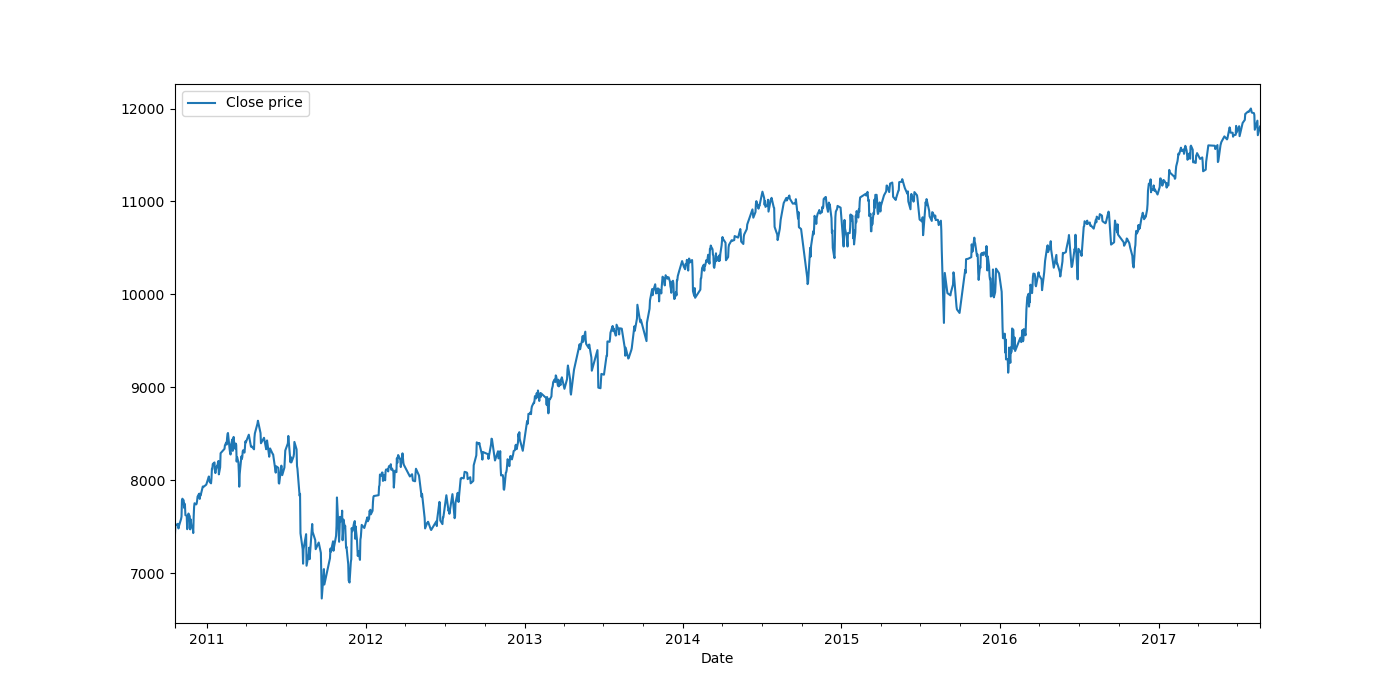
\includegraphics[width=\textwidth]{figures/Ass2/Ass2_Q2_raw_signal.png}
    \end{minipage}
    \caption{The raw signal of the dataset.}
    \label{fig:Ass2_Q2_raw_signal}
\end{figure}

\begin{figure}[H]
    \centering
    \begin{minipage}[b]{1\textwidth}
        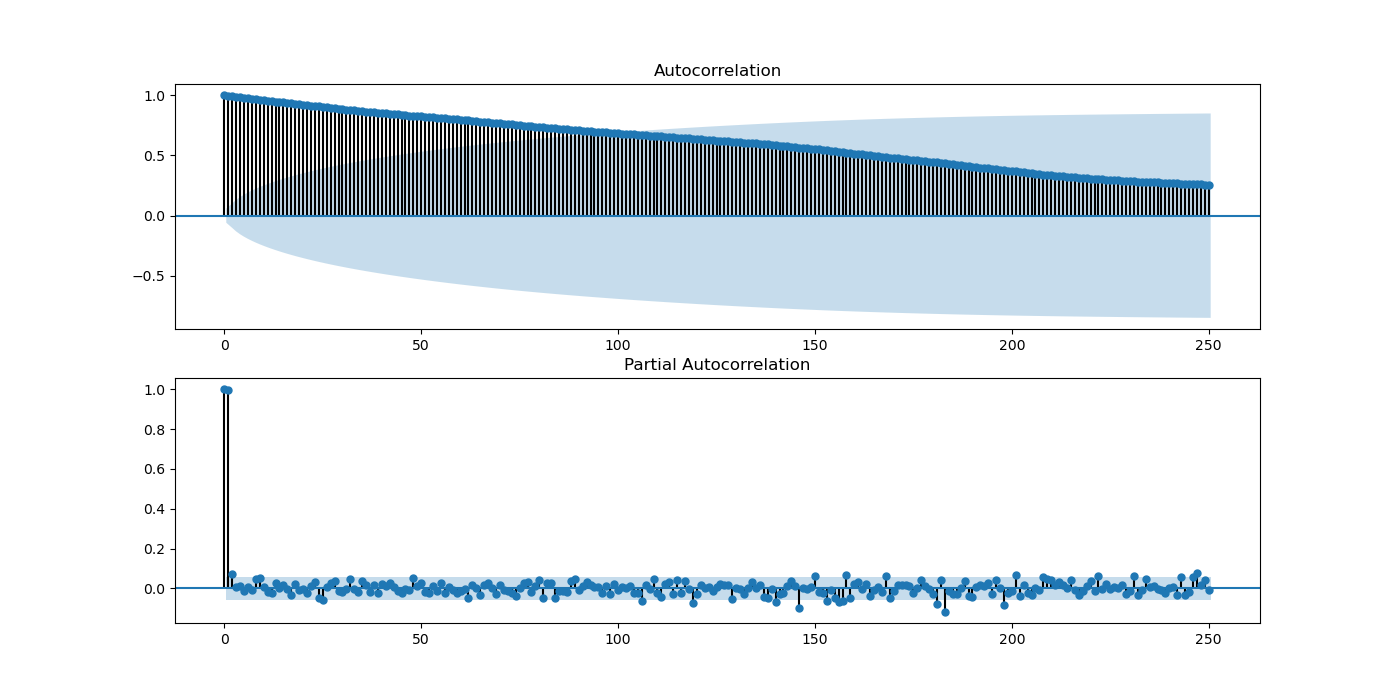
\includegraphics[width=\textwidth]{figures/Ass2/Ass2_Q2_PACF_ACF.png}
    \end{minipage}
    \caption{A plot of \gls{ACF} and \gls{PACF} of the dataset.}
    \label{fig:Ass2_Q2_PACF_ACF}
\end{figure}


\textit{Figures \ref{fig:Ass2_Q2_raw_signal} and \ref{fig:Ass2_Q2_PACF_ACF} indicate the raw signal along with its \gls{ACF} and \gls{PACF} plots. \gls{ACF} and \gls{PACF} plots allow us to determine how correlated points are with each other. Furthermore, the period of the seasonal component can calculate by \gls{ACF}. As can be seen, the \gls{ACF} plot has no oscillation. Therefore there is no seasonal component related to our time series.}




\textit{In order to turn the dataset into a stationary dataset, we used a first-order differencing. Table \ref{tab:Ass2_Q2_ADF_1diff} indicates the result of \gls{ADF}  on the first-order differencing. As this test shows, the data got a stationary data. Figures \ref{fig:Ass2_Q2_1diff_signal} and \ref{fig:Ass2_Q2_PACF_ACF_1diff} indicate the $1^{st}$ order differencing signal along with its \gls{ACF} and \gls{PACF} plots. These two plots also show that the data is stationary. }

\begin{table}[H]
\centering
\caption{The result of the \gls{ADF} on the $1^{st}$ order differencing in the dataset.}
\label{tab:Ass2_Q2_ADF_1diff}
\begin{tabular}{lr}
\toprule
{} &            0 \\
\midrule
ADF Statistic               &   -25.690334 \\
p-value                     &     0.000000 \\
\#Lags Used                  &     1.000000 \\
Number of Observations Used &  1111.000000 \\
Critical Value (1\%)         &    -3.436250 \\
Critical Value (5\%)         &    -2.864145 \\
Critical Value (10\%)        &    -2.568157 \\
\bottomrule
\end{tabular}

\end{table}

\begin{figure}[H]
    \centering
    \begin{minipage}[b]{1\textwidth}
        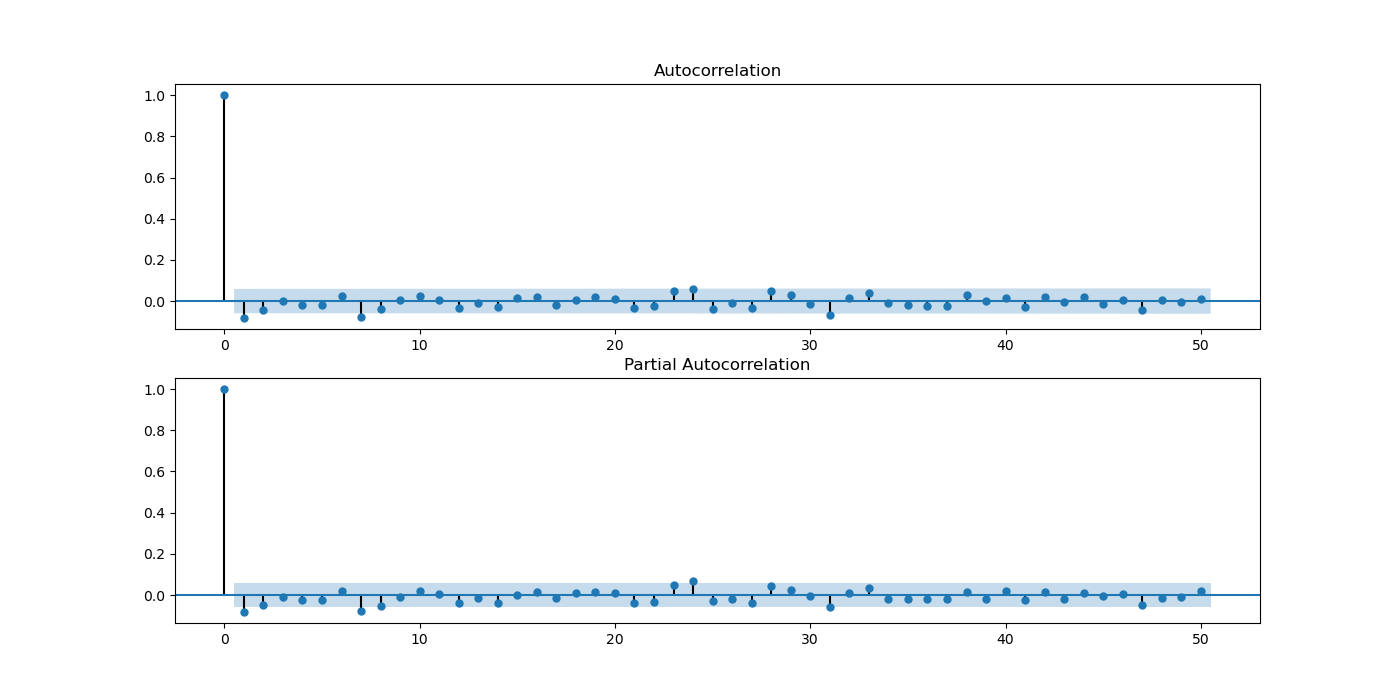
\includegraphics[width=\textwidth]{manuscript/src/figures/Ass2/Ass2_Q2_PACF_ACF_1diff.png}
    \end{minipage}
    \caption{ A plot of the \gls{ACF} and \gls{PACF} on the $1^{st}$ order differencing in the dataset.}
    \label{fig:Ass2_Q2_PACF_ACF_1diff}
\end{figure}
\begin{figure}[H]
    \centering
    \begin{minipage}[b]{1\textwidth}
        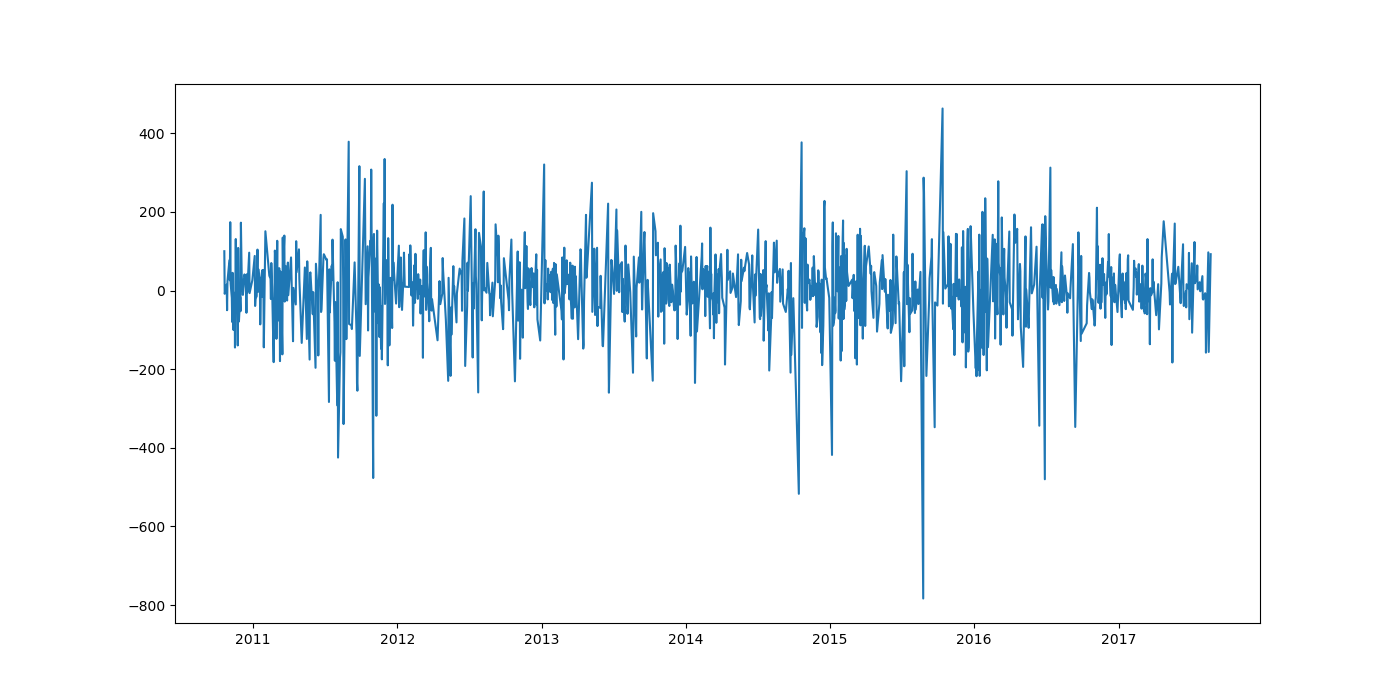
\includegraphics[width=\textwidth]{manuscript/src/figures/Ass2/Ass2_Q2_1diff_signal.png}
    \end{minipage}
    \caption{ The signal of $1^{st}$ order differencing.}
    \label{fig:Ass2_Q2_1diff_signal}
\end{figure}



\textit{We used grid search and interpreting \gls{ACF} and \gls{PACF} plots to select the best order for \gls{arima}.}

\textit{Since both \gls{ACF} and \gls{PACF} (see figure \ref{fig:Ass2_Q2_PACF_ACF_1diff}) had one significant lag, it concluded that both AR order (q) and MA order (p) were one. Also, based on using $1^{st}$ order differencing, the integrated order (d) set 1.}

\textit{In grid search, we set a space search to find the model that had the lowest error. Table \ref{tab:ass2_Q2_1} shows our space search. This method selected the order \gls{arima}(1, 1, 1) as the best-fitted model.}

\begin{table}[H]
\centering
\caption{The space search of grid search.}
\label{tab:ass2_Q2_1}
\begin{tabular}{lcc}
\toprule
\# & hyper-parameter      & values\\ \hline
\midrule

1 & p & $1 \thicksim 4$               \\ \hline
2 & q & $1 \thicksim 4$               \\ \hline
3 & d & 1               \\ \hline
\bottomrule
\end{tabular}
\end{table}

\textit{Figure \ref{fig:Ass2_Q2_best_model_residual} indicates the residual of the best-fitted model. As this plot illustrates, the residual signal had a Gaussian distribution with zero mean. Besides, the \gls{ACF} plot shows that this signal was stationary.}



\begin{figure}[H]
    \centering
    \begin{minipage}[b]{1\textwidth}
        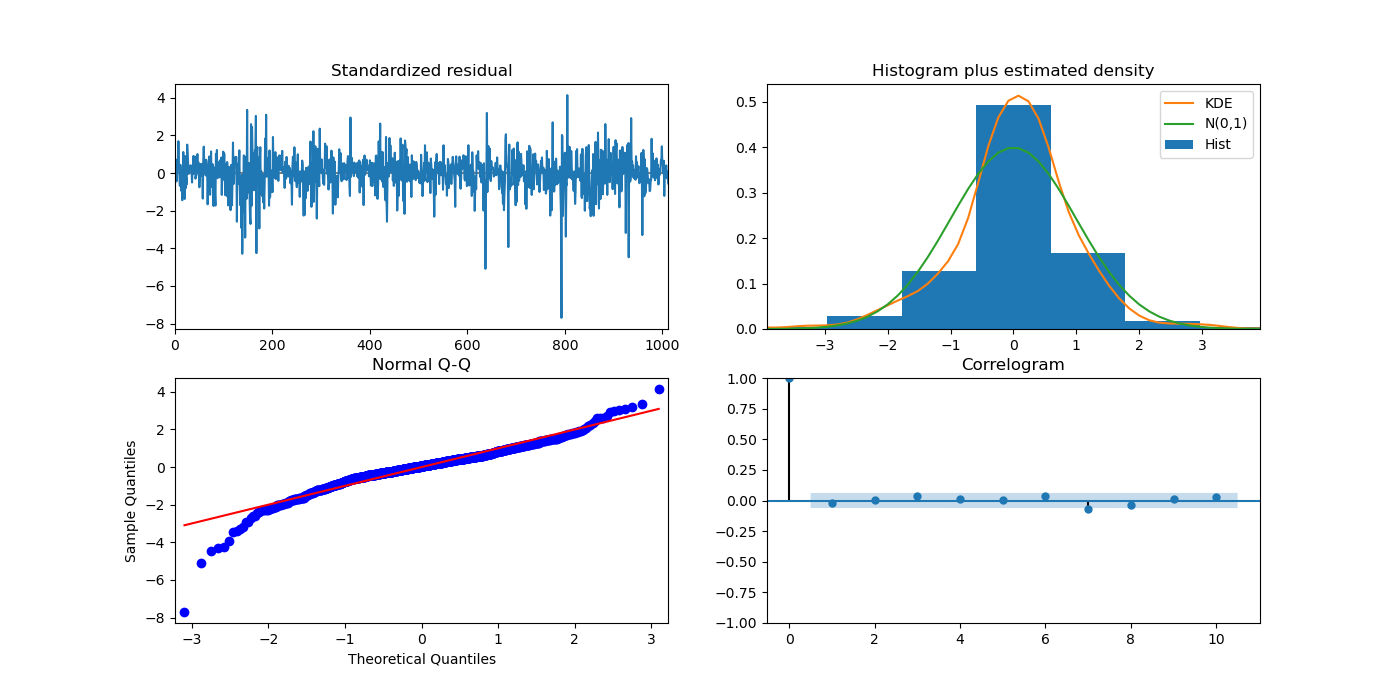
\includegraphics[width=\textwidth]{manuscript/src/figures/Ass2/Ass2_Q2_best_model_residual.png}
    \end{minipage}
    \caption{The residual  of the best-fitted model (\gls{arima}(1, 1, 1)) based on grid search.}
    \label{fig:Ass2_Q2_best_model_residual}
\end{figure}

  
\textit{To predict, we split data into test and train sets. We considered about 35 samples for the test set and others for training. Figure \ref{fig:Ass2_Q2_Automatic_model_forcasting} demonstrates the output of the best-fitted model. As can be seen, the model could predict the upward trend. The obtained RMS error was 294.506. Although this model could predict the first sample, it could not follow the rest perfectly.}

\begin{figure}[H]
    \centering
    \begin{minipage}[b]{1\textwidth}
        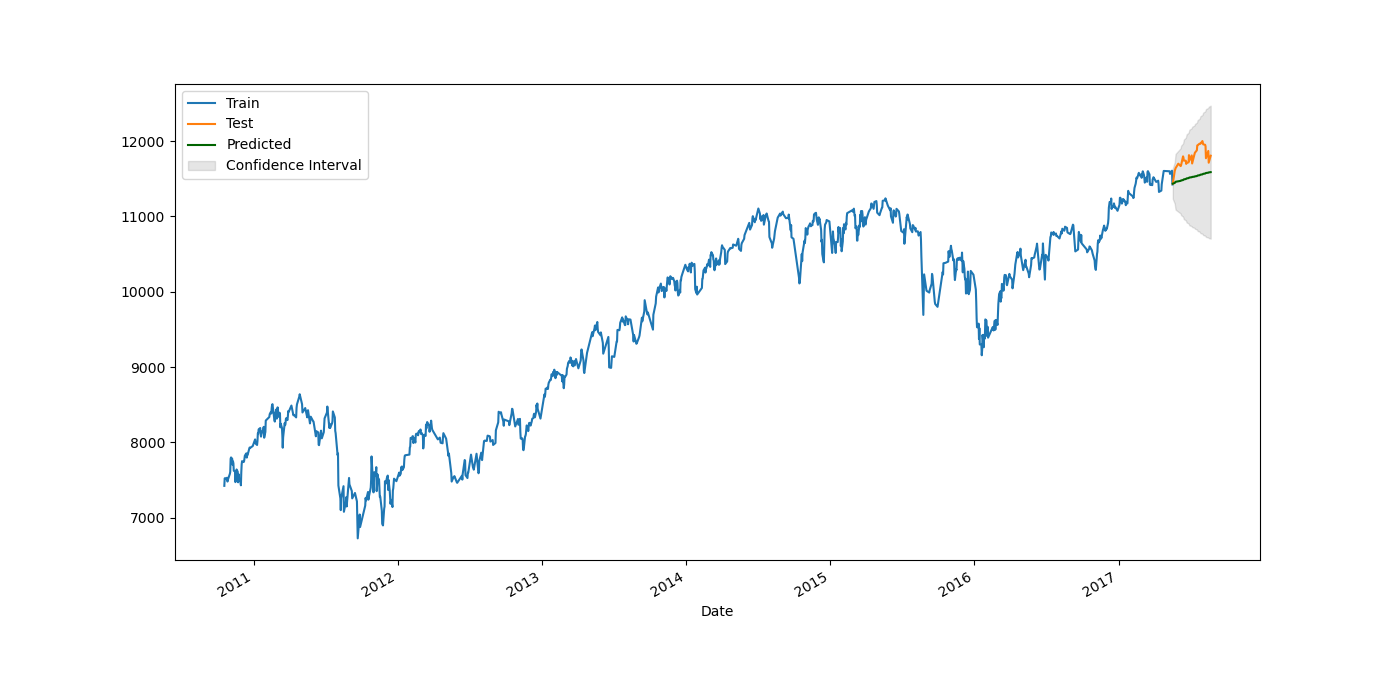
\includegraphics[width=\textwidth]{manuscript/src/figures/Ass2/Ass2_Q2_Automatic_model_forcasting.png}
    \end{minipage}
    \caption{The prediction and actual data of \gls{arima}(1, 1, 1) model.}
    \label{fig:Ass2_Q2_Automatic_model_forcasting}
\end{figure}


\textit{For the rolling window approach, we predicted only one day. Then the actual value of this day was added to the training set while our training set had a fixed size. We considered 500 samples (three years). The figure below shows the training set.}
\begin{figure}[H]
    \centering
    \begin{minipage}[b]{1\textwidth}
        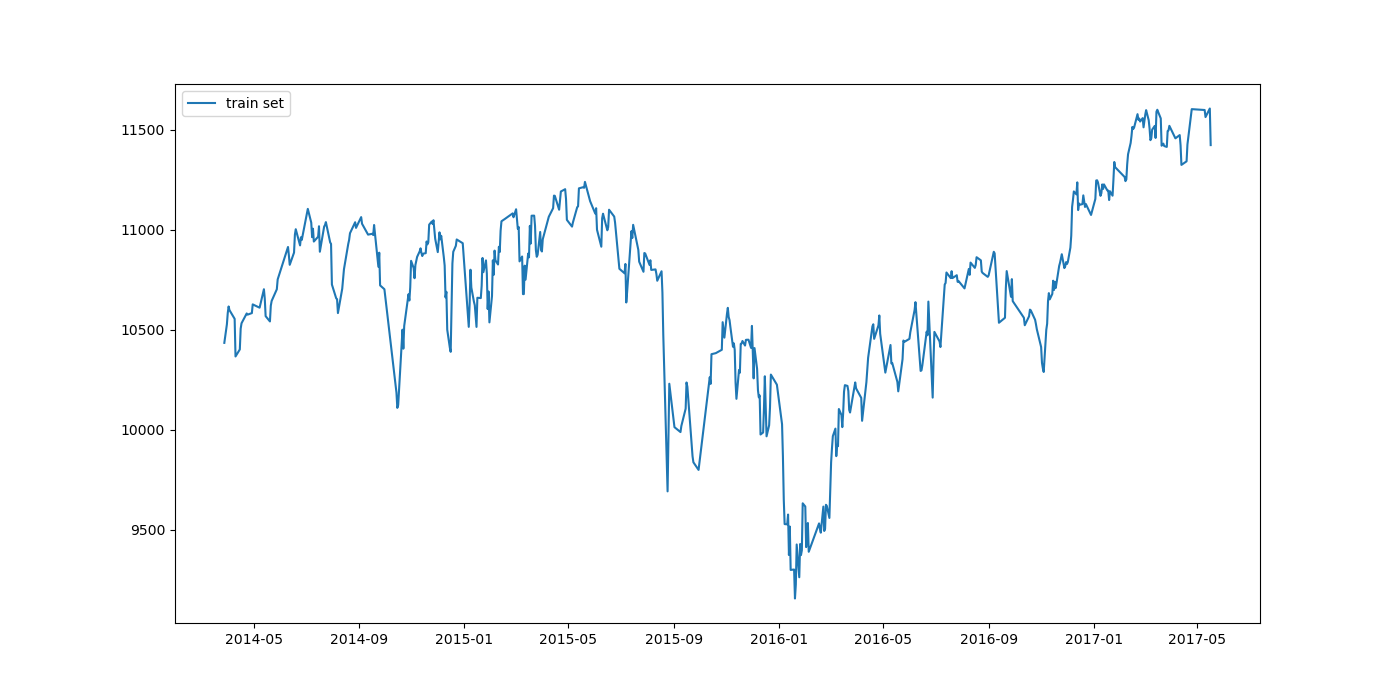
\includegraphics[width=\textwidth]{manuscript/src/figures/Ass2/Ass2_Q2_Rolling_trainset.png}
    \end{minipage}
    \caption{The training set for rolling window approach.}
    \label{fig:Ass2_Q2_Rolling_trainset}
\end{figure}

\textit{Since the training set did not change, we used the same order of the last model. Figures \ref{fig:Ass2_Q2_Rolling_Forecast} and \ref{fig:Ass2_Q2_Rolling_Forecast_1} demonstrate the output of the rolling window model. As can be seen, the model could follow the test set. Besides, the RMS error reduced from 294.506 to 69.371.}

\begin{figure}[H]
    \centering
    \begin{minipage}[b]{1\textwidth}
        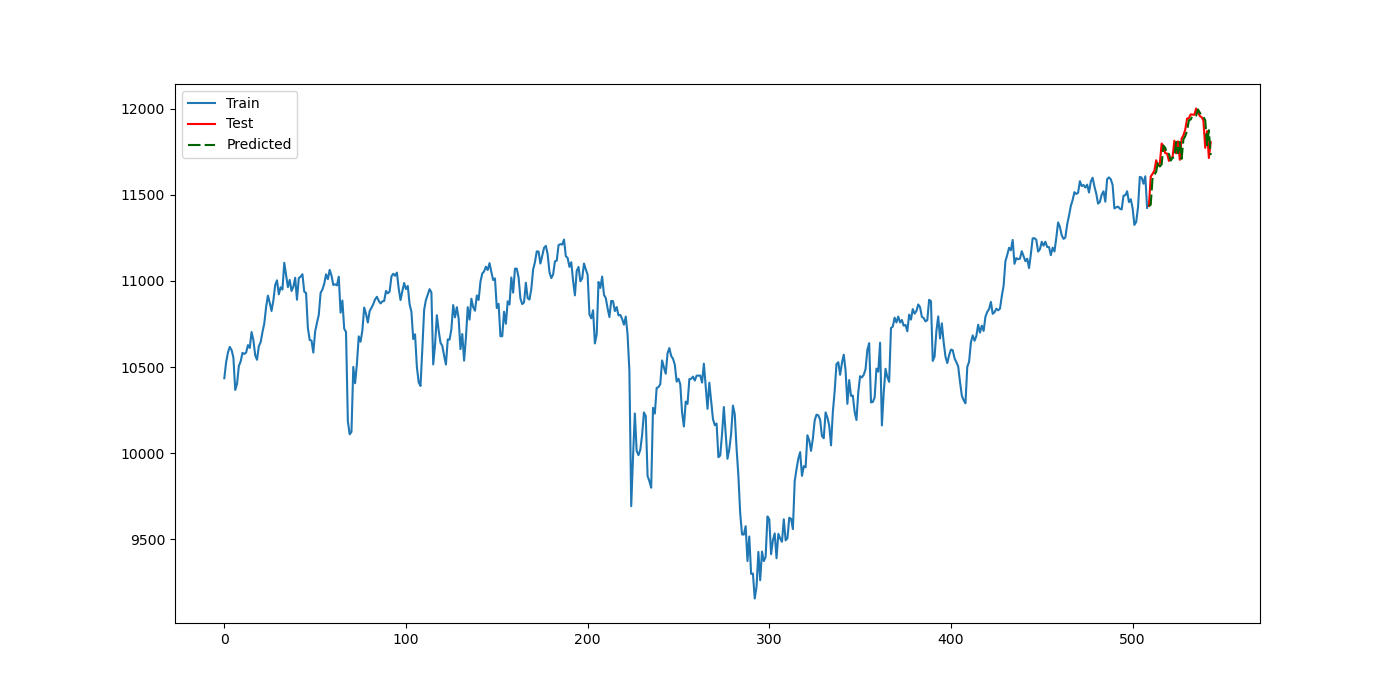
\includegraphics[width=\textwidth]{manuscript/src/figures/Ass2/Ass2_Q2_Rolling_Forecast_1.png}
    \end{minipage}
    \caption{The prediction and actual data of \gls{arima}(1, 1, 1) model in rolling windows approach.}
    \label{fig:Ass2_Q2_Rolling_Forecast_1}
\end{figure}

\begin{figure}[H]
    \centering
    \begin{minipage}[b]{1\textwidth}
        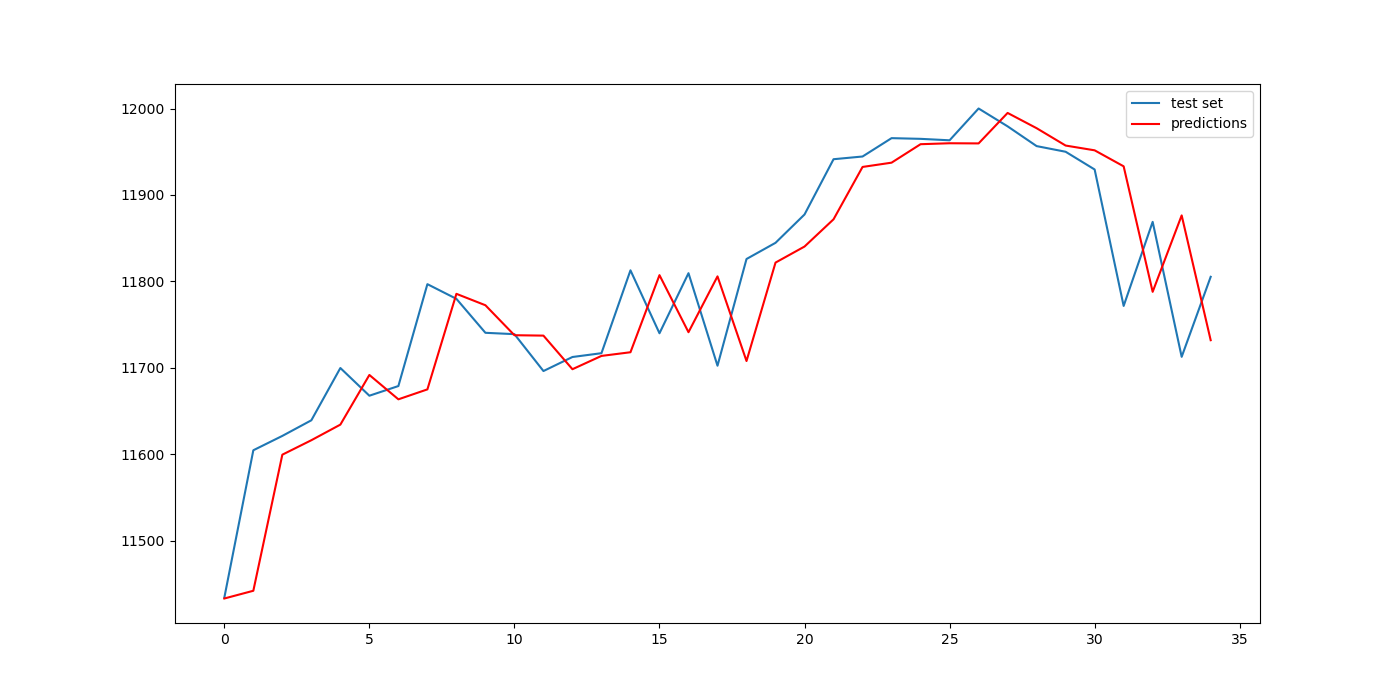
\includegraphics[width=\textwidth]{manuscript/src/figures/Ass2/Ass2_Q2_Rolling_Forecast.png}
    \end{minipage}
    \caption{The prediction and test set of \gls{arima}(1, 1, 1) model in rolling windows approach.}
    \label{fig:Ass2_Q2_Rolling_Forecast}
\end{figure}





%%%%%%%%%%%%%%%%%%%%%%%%%%%%%%%%%%%%%%%%%%%%%%%%%%%%%%%%%%%%%%%%%
%%%%%%%%%%%%%%%%%%%%%%%% Question 2 %%%%%%%%%%%%%%%%%%%%%%%%%%%%%
%%%%%%%%%%%%%%%%%%%%%%%%%%%%%%%%%%%%%%%%%%%%%%%%%%%%%%%%%%%%%%%%%
\newpage
\item \textbf{Now, explore whether you can leverage additional information in the file as exogenous variables. Use appropriate tools to evaluate the suitability of using these variables and summarize your results. There is no fixed number of variables assigned – use your judgement and justify your decisions.  Using an ARIMAX framework, show the impact of including additional variables as part of your prediction. Repeat the analysis in 2 (a) and (b) using the updated models.} 


\textit{First, we visualized the raw signals.} 

\begin{figure}[H]
    \centering
    \begin{minipage}[b]{1\textwidth}
        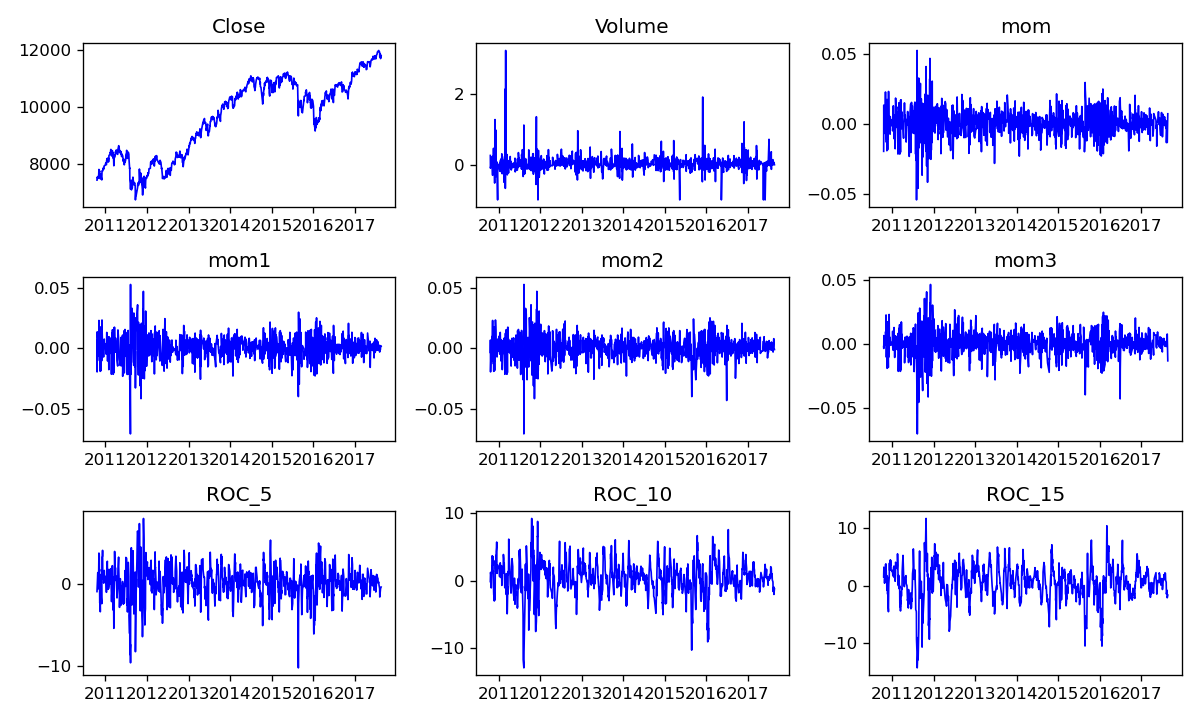
\includegraphics[width=\textwidth]{figures/Ass2/Ass2_Q3_raw_signal.png}
    \end{minipage}
    \caption{The visualization of the first nine columns.}
    \label{fig:Ass2_Q3_raw_signal}
\end{figure}


\textit{Before any transformation, we applied the Granger causality test on the first 20 variables. The null hypothesis (H0) of this test says that two variables do not Granger causes, and its alternate hypothesis (H1) indicates the second signal has a significant effect on the first signal. So, wherever P-value is less than 0.05, we can consider Grange causality. Table \ref{tab:Ass2_Q3_Granger_results1} indicates the result of this test on the first twelve columns. For this test, the maximum lag set 12.\\
Based on this test, signals mom, mom1, ROC\_X, Oil, and EMA\_X were Granger causality of the "Close price"; We stored these variables for the next steps. }

\begin{table}[H]
\centering
\caption{The result of Granger causality test.}
\label{tab:Ass2_Q3_Granger_results1}
\begin{tabular}{rlrrc}
\toprule
\# & Variable Name &  min\_p\_value &   lag &  Causality \\
\midrule
1 & Close   &       1.0000 &   1.0 &        - \\
2 & Volume  &       0.2613 &  10.0 &        - \\
3 & mom     &       0.0022 &   8.0 &        \Tik \\
4 & mom1    &       0.0285 &   7.0 &        \Tik \\
5 & mom2    &       0.2049 &   2.0 &        - \\
6 & mom3    &       0.0860 &   1.0 &        - \\
7 & ROC\_5   &       0.0024 &   1.0 &        \Tik \\
8 & ROC\_10  &       0.0036 &   1.0 &        \Tik \\
9 & ROC\_15  &       0.0037 &   1.0 &        \Tik \\
10 & ROC\_20  &       0.0010 &   9.0 &        \Tik \\
11 & EMA\_10  &       0.0021 &   1.0 &        \Tik \\
12 & EMA\_20  &       0.0014 &   1.0 &        \Tik \\
13 & EMA\_50  &       0.0008 &   9.0 &        \Tik \\
14 & EMA\_200 &       0.0035 &   9.0 &        \Tik \\
15 & DTB4WK  &       0.2096 &   1.0 &        - \\
16 & DTB3    &       0.1918 &   1.0 &        - \\
17 & DTB6    &       0.2826 &  10.0 &        - \\
18 & DGS5    &       0.5876 &   5.0 &        - \\
19 & DGS10   &       0.3805 &   5.0 &        - \\
20 & Oil     &       0.0120 &   7.0 &        \Tik \\
\bottomrule
\end{tabular}

\end{table}

\textit{As these signals had a different range, we used standardization to transform all data to scale -1 and 1. Figure \ref{fig:Ass2_Q3_standard_data} indicates the standardized variables. Also, we applied \gls{ADF} on these signals to find out that these signals were stationary or non-stationary. Table \ref{tab:Ass2_Q3_ADF_results} shows the result of this test on the dataset.}

\begin{figure}[H]
    \centering
    \begin{minipage}[b]{1\textwidth}
        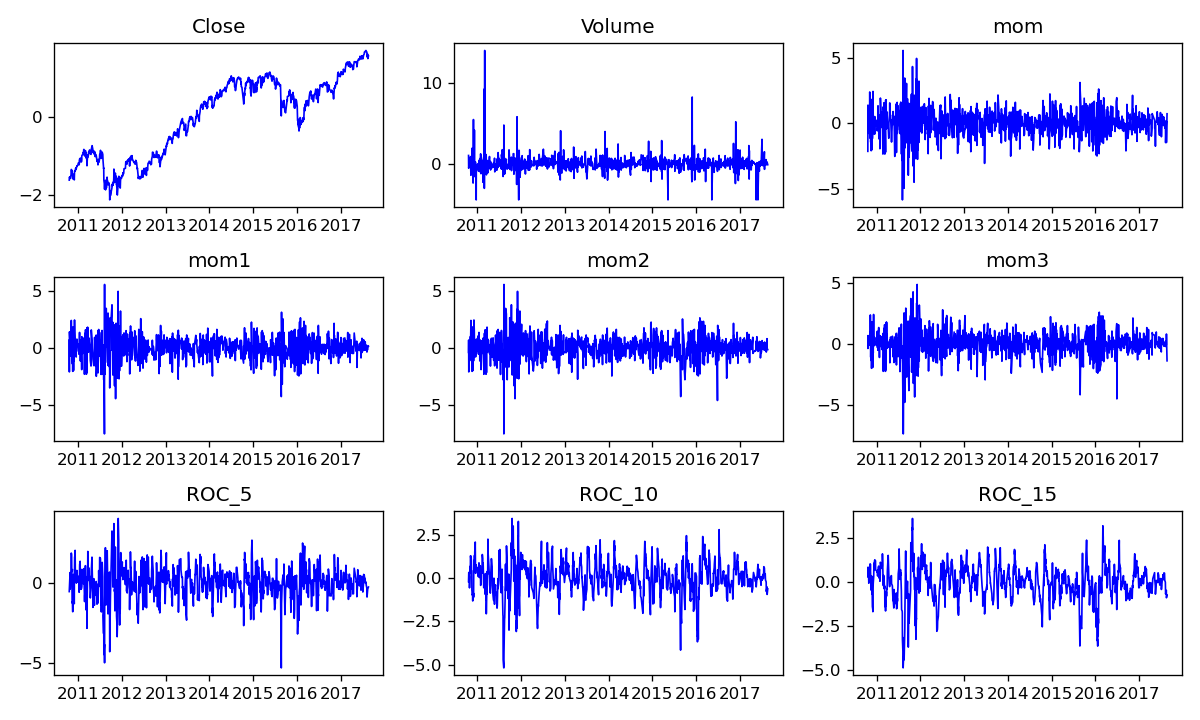
\includegraphics[width=\textwidth]{figures/Ass2/Ass2_Q4_standard_data.png}
    \end{minipage}
    \caption{The visualization of the first twelve columns. Columns were standardized.}
    \label{fig:Ass2_Q3_standard_data}
\end{figure}



\begin{table}[H]
\centering
\caption{The result of the \gls{ADF} on the dataset.}
\label{tab:Ass2_Q3_ADF_results}
{\tiny
\hspace*{-2cm}\begin{tabular}{lrrrrrrrrrrrr}
\toprule
{} &        Close &           mom &         mom1 &         ROC\_5 &        ROC\_10 &        ROC\_15 &        ROC\_20 &       EMA\_10 &       EMA\_20 &       EMA\_50 &      EMA\_200 &           Oil \\
\midrule
ADF Statistic               &    -1.085 & -12.134 &   -38.465 & -10.619 & -9.753 & -6.995 & -8.074 &    -0.967 &    -0.882 &    -0.791 &    -0.585 & -8.920 \\
p-value                     &     0.7 &  1.7e-22 &     0 &  5.5e-19 &  7.9e-17 &  7.5e-10 &  1.5e-12 &     0.7 &     0.7 &     0.8 &     0.8 &  1.0e-14 \\
\# Lags Used                  &     2 &  11 &     0 &  9 &  6 &  16 &  5 &     3 &     3 &     6 &     7 &  10 \\
\# Obs. Used &  1111 &  1102 &  1113 &  1104 &  1107 &  1097 &  1108 &  1110 &  1110 &  1107 &  1106 &  1103 \\
Critical Value (1\%)         &    -3.436 & -3.436 & -3.436 &    -3.436 & -3.436 &    -3.436 & -3.436 & -3.436 & -3.436 & -3.436 & -3.436 & -3.436 \\
Critical Value (5\%)         &    -2.864 & -2.864 & -2.864 &    -2.864 & -2.864 &    -2.864 & -2.864 & -2.864 & -2.864 & -2.864 & -2.864 & -2.864 \\
Critical Value (10\%)        &    -2.568 & -2.568 & -2.568 &    -2.568 & -2.568 &    -2.568 & -2.568 & -2.568 & -2.568 & -2.568 & -2.568 & -2.568\\
\bottomrule
\end{tabular}\hspace*{-2cm}
}
\end{table}

\textit{According to table \ref{tab:Ass2_Q3_ADF_results} all columns were stationary except the "Close price" and EMA\_X variables. Therefore, 
we used a first-order differencing to turn these time series into the stationary data. Figures \ref{fig:Ass2_Q3_1diff_Close_signal} and \ref{fig:Ass2_Q3_PACF_ACF_1diff} indicate this $1^{st}$ order differencing on "Close price" along with its \gls{ACF} and \gls{PACF} plots. These two plots also show that the data got stationary. Also, table \ref{tab:Ass2_Q3_ADF_results2} shows the ADF test on the $1^{st}$ order differencing variables.}

\begin{figure}[H]
    \centering
    \begin{minipage}[b]{1\textwidth}
        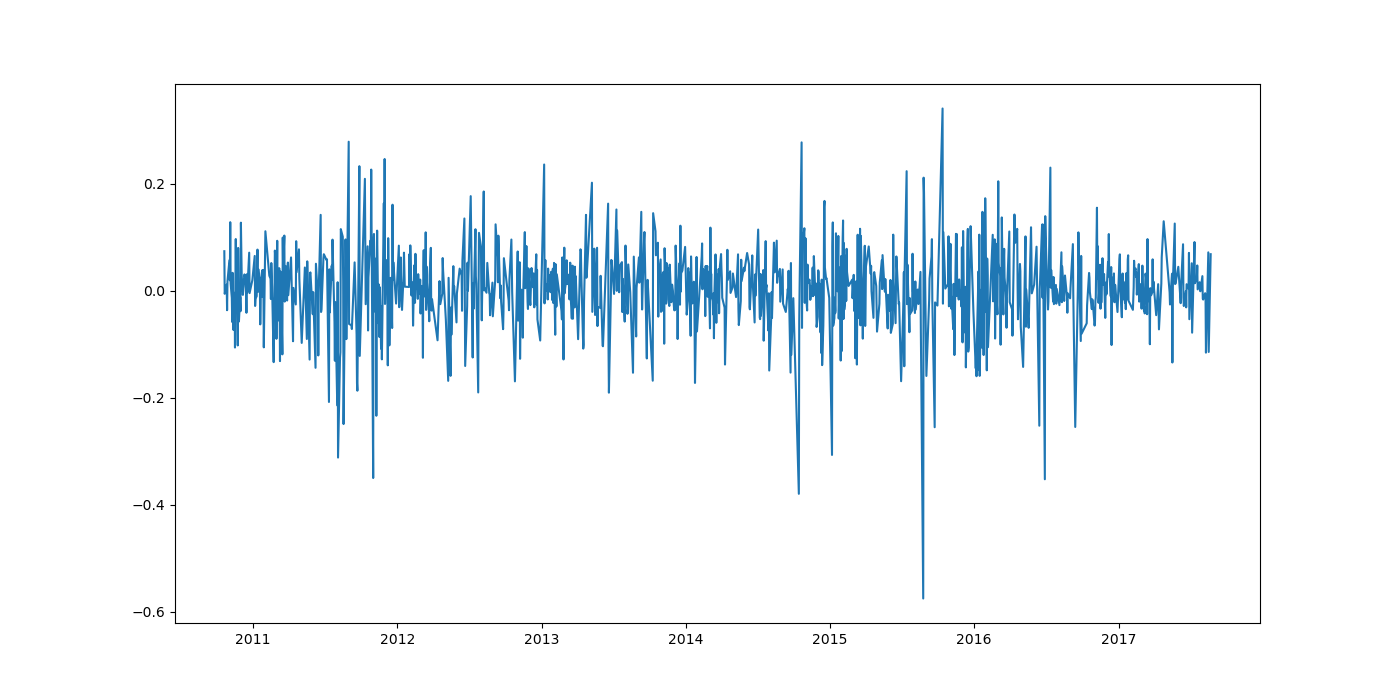
\includegraphics[width=\textwidth]{figures/Ass2/Ass2_Q3_1diff_Close_signal.png}
    \end{minipage}
    \caption{The $1^{st}$ order differencing of "Close price" data.}
    \label{fig:Ass2_Q3_1diff_Close_signal}
\end{figure}

\begin{figure}[H]
    \centering
    \begin{minipage}[b]{1\textwidth}
        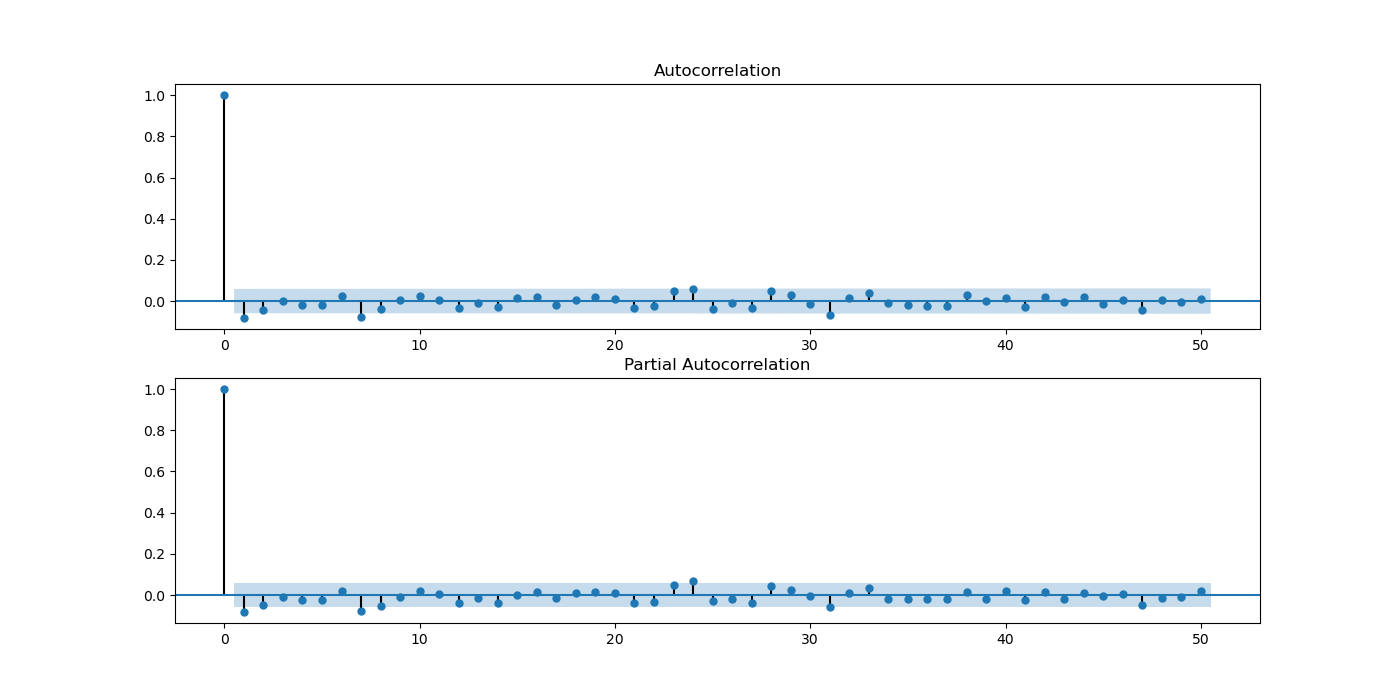
\includegraphics[width=\textwidth]{figures/Ass2/Ass2_Q3_PACF_ACF_1diff.png}
    \end{minipage}
    \caption{A plot of \gls{ACF} and \gls{PACF} on the $1^{st}$ order differencing in "Close price".}
    \label{fig:Ass2_Q3_PACF_ACF_1diff}
\end{figure}

\begin{table}[H]
\centering
\caption{The result of the \gls{ADF} on the $1^{st}$ order differencing variables.}
\label{tab:Ass2_Q3_ADF_results2}
{\tiny
\hspace*{-2cm}\begin{tabular}{lrrrrrrrrrrrr}
\toprule
{} &        Close &           mom &         mom1 &         ROC\_5 &        ROC\_10 &        ROC\_15 &        ROC\_20 &       EMA\_10 &       EMA\_20 &       EMA\_50 &      EMA\_200 &           Oil \\
\midrule
ADF Statistic               &   -25.69 & -12.13 &   -24.15 & -10.63 & -9.74 & -6.99 & -8.059 & -13.44 & -10.72 & -6.82 &    -4.72 & -8.91 \\

p-value                     &     0 &  1.7e-22 &     0 &  4.9e-19 &  8.1e-17 &  7.4e-10 &  1.6e-12 &  3.7e-25 &  3.0e-19 &  1.9e-09 &     7.6e-5 &  1.0e-14 \\
\#Lags Used                  &     1 &  11 &     1 &  9 &  6 &  16 &  5 &  2 &  2 &  5 &     6 &  10 \\
\# Observations Used &  1111 &  1101 &  1111 &  1103 &  1106 &  1096 &  1107 &  1110 &  1110 &  1.107 &  1106 &  1102 \\
Critical Value (1\%)         &    -3.436 & -3.436 & -3.436 &    -3.436 & -3.436 &    -3.436 & -3.436 & -3.436 & -3.436 & -3.436 & -3.436 & -3.436 \\
Critical Value (5\%)         &    -2.864 & -2.864 & -2.864 &    -2.864 & -2.864 &    -2.864 & -2.864 & -2.864 & -2.864 & -2.864 & -2.864 & -2.864 \\
Critical Value (10\%)        &    -2.568 & -2.568 & -2.568 &    -2.568 & -2.568 &    -2.568 & -2.568 & -2.568 & -2.568 & -2.568 & -2.568 & -2.568\\
\bottomrule
\end{tabular}\hspace*{-2cm}
}
\end{table}

\textit{After transforming and making stationary, we needed to shift exogenous variables as much as the corresponding lag in the Granger causality result.}

\textit{We fitted our model based on exogenous variables. The order of the model for this question was similar to the last question. Figure \ref{fig:Ass2_Q3_residual_plot} indicates the residual of the fitted model. As this plot illustrates, the residual signal of the model had a Gaussian distribution with zero mean. Besides, the \gls{ACF} plot shows that this signal is stationary.}



\begin{figure}[H]
    \centering
    \begin{minipage}[b]{1\textwidth}
        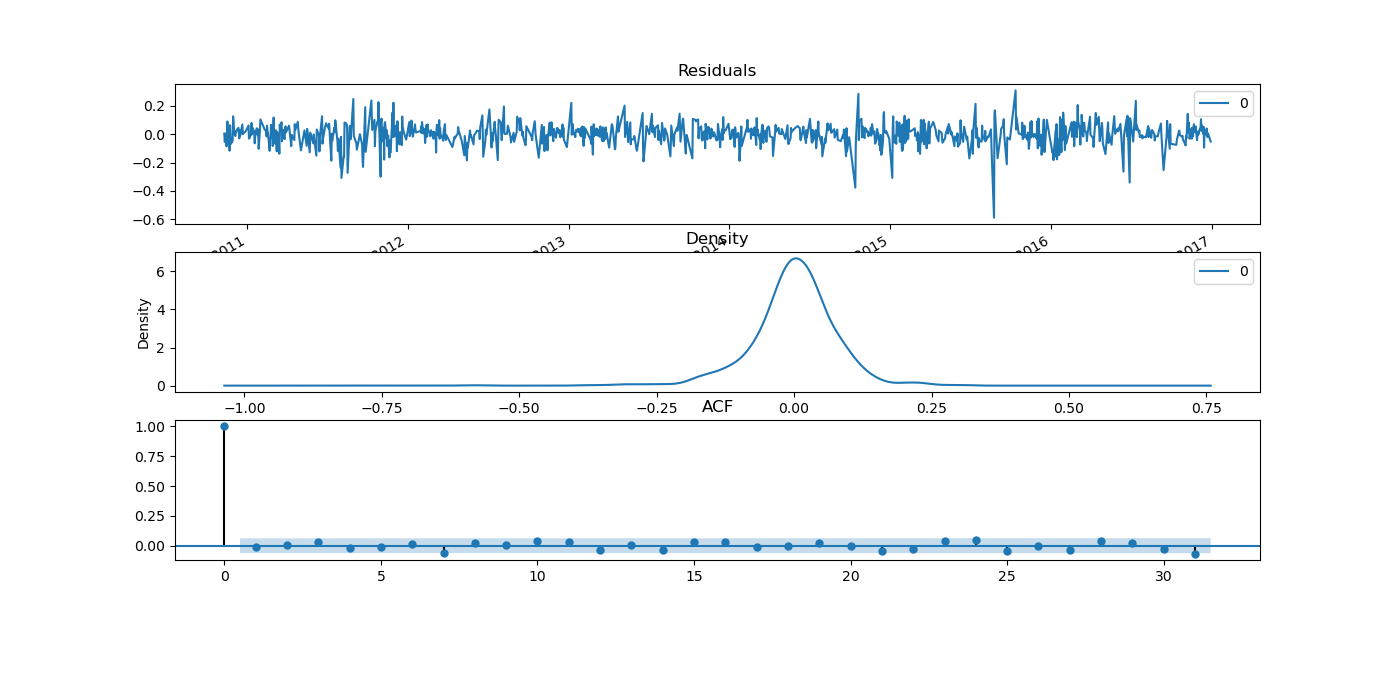
\includegraphics[width=\textwidth]{manuscript/src/figures/Ass2/Ass2_Q3_residual_plot.png}
    \end{minipage}
    \caption{The residual of the fitted model (\gls{arima}X(1, 0, 1)).}
    \label{fig:Ass2_Q3_residual_plot}
\end{figure}

\textit{To forecast, we split data into test and train set like part 2. After prediction, we needed to reverse all transformations to get the real forecast. Figure \ref{fig:Ass2_Q3_Forecast_vs_Actuals} demonstrates the output of the fitted model. As can be seen, because of using the exogenous variables, the model could predict some changes, and for others could not follow the actual data. The RMS error was 328.647.} 

\begin{figure}[H]
    \centering
    \begin{minipage}[b]{1\textwidth}
        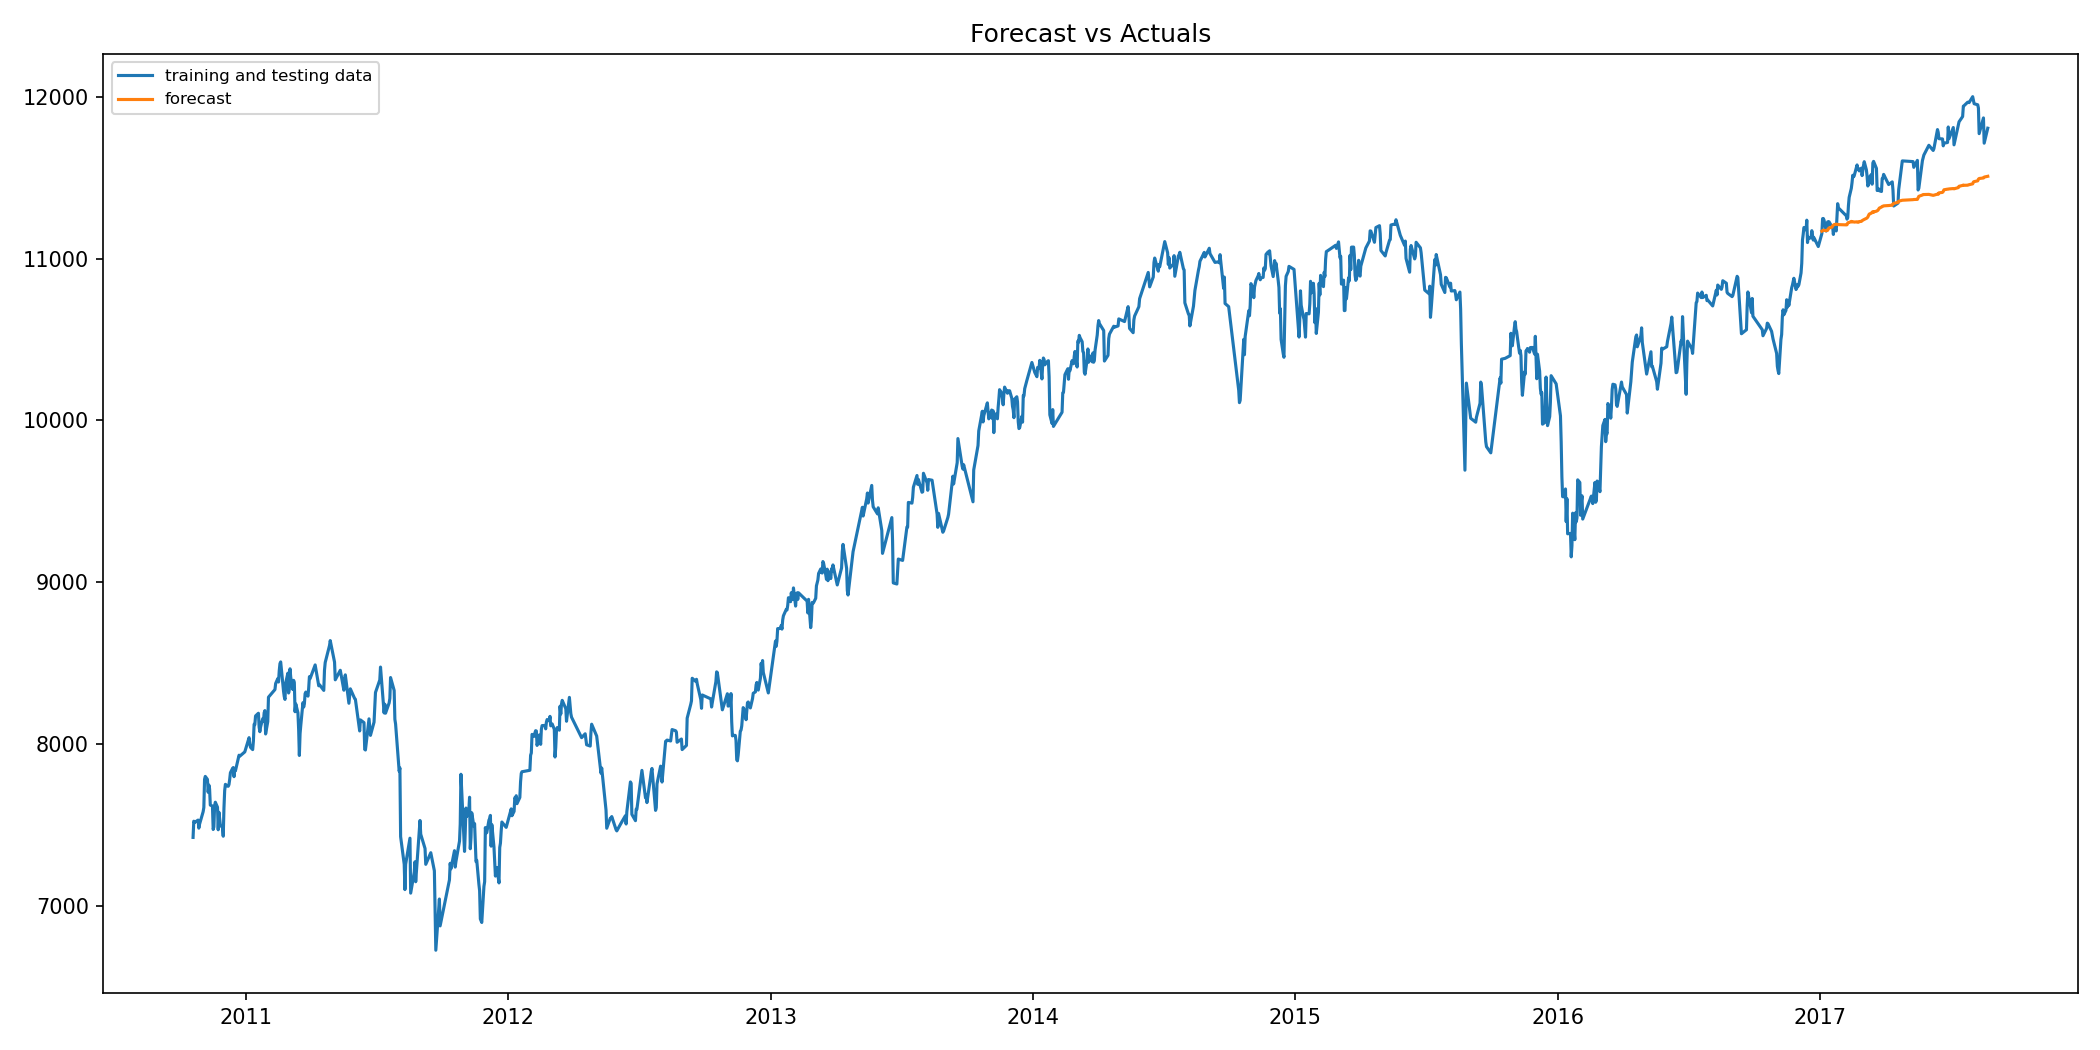
\includegraphics[width=\textwidth]{manuscript/src/figures/Ass2/Ass2_Q3_Forecast_vs_Actuals.png}
    \end{minipage}
    \caption{The prediction and actual data of \gls{arima}X(1, 0, 1) model.}
    \label{fig:Ass2_Q3_Forecast_vs_Actuals}
\end{figure}





\textit{For the rolling window approach, we used the same procedure in question 2. Figure \ref{fig:Ass2_Q3_Rolling_Forecast_vs_Actuals} demonstrates the output of the rolling window model for \gls{arima}X. As can be seen, the model could follow the test set better than previous model. The RMS error decreased from 328.647 to 256.297. It seems that the prediction of both models had a negative bias.}

\begin{figure}[H]
    \centering
    \begin{minipage}[b]{1\textwidth}
        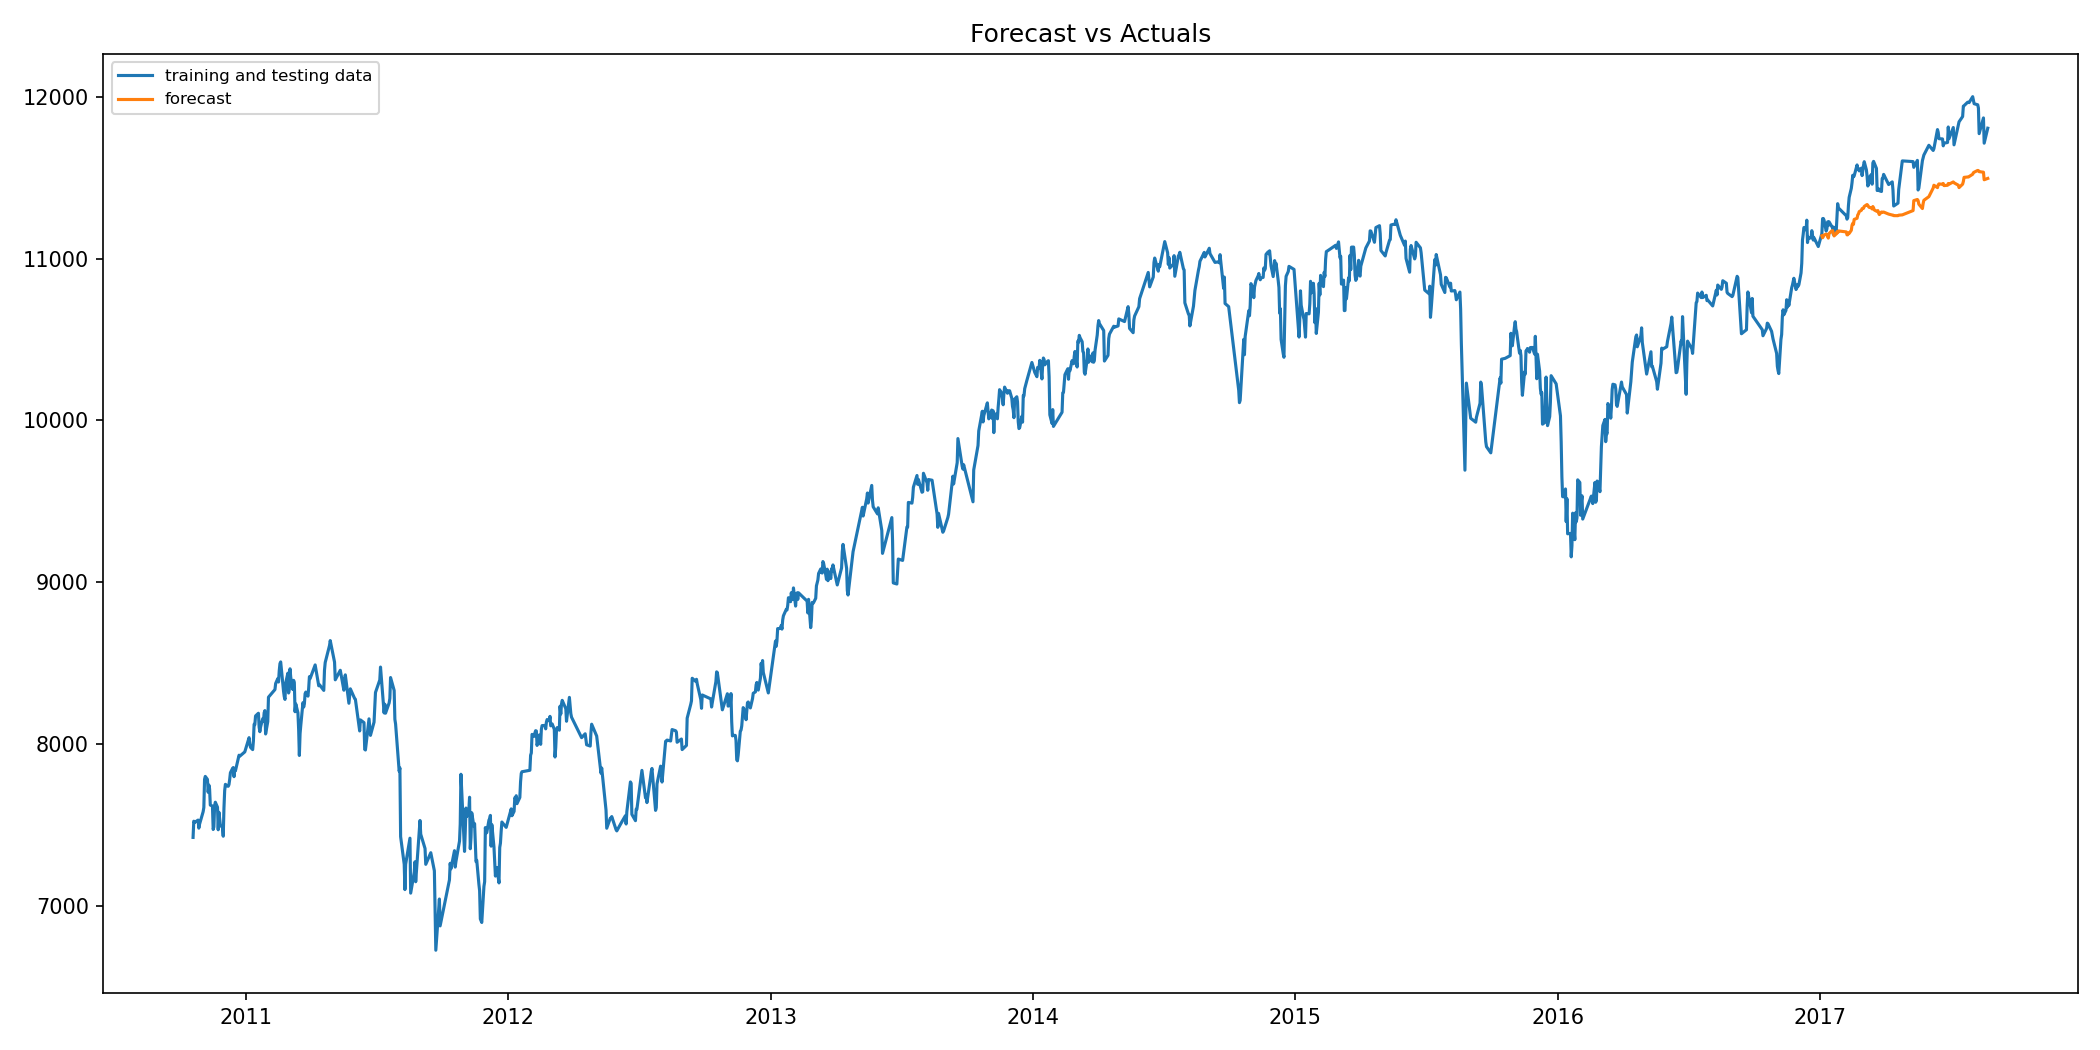
\includegraphics[width=\textwidth]{manuscript/src/figures/Ass2/Ass2_Q3_Rolling_Forecast_vs_Actuals.png}
    \end{minipage}
    \caption{The prediction and actual data of \gls{arima}X(1, 0, 1) model in rolling windows approach.}
    \label{fig:Ass2_Q3_Rolling_Forecast_vs_Actuals}
\end{figure}









%%%%%%%%%%%%%%%%%%%%%%%%%%%%%%%%%%%%%%%%%%%%%%%%%%%%%%%%%%%%%%%%%
%%%%%%%%%%%%%%%%%%%%%%%% Question 3 %%%%%%%%%%%%%%%%%%%%%%%%%%%%%
%%%%%%%%%%%%%%%%%%%%%%%%%%%%%%%%%%%%%%%%%%%%%%%%%%%%%%%%%%%%%%%%%
\newpage
\item \textbf{Finally, repeat the analysis in 3 but for a VAR-based approach. Explore the relationships between the chosen variables using appropriate tools. Again, there is no fixed number of variables assigned – use your judgement and justify your decisions.  Using a VAR framework, show the impact of including additional variables in your prediction. Repeat the analysis in 2 (a) and (b) using the updated models.} 

\textit{Likewise the last question, we visualized the first nine signals to see what kind of data we have.} 

\begin{figure}[H]
    \centering
    \begin{minipage}[b]{1\textwidth}
        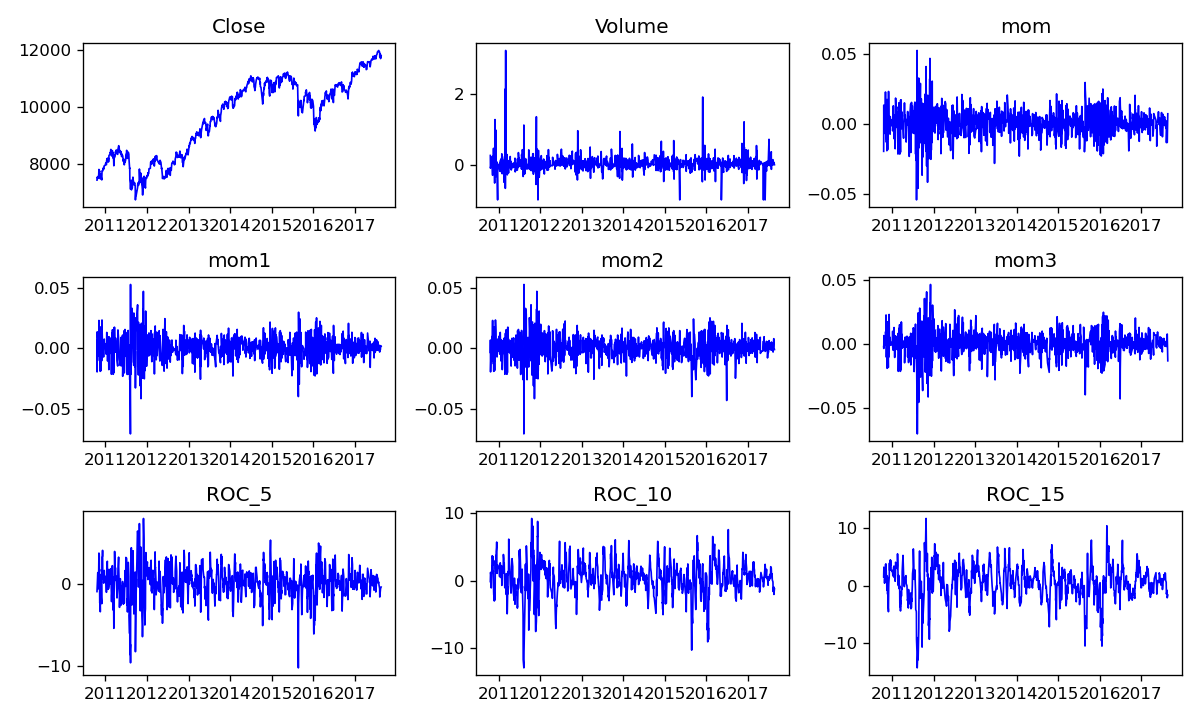
\includegraphics[width=\textwidth]{figures/Ass2/Ass2_Q3_raw_signal.png}
    \end{minipage}
    \caption{The visualization of the first nine columns.}
    \label{fig:Ass2_Q4_raw_signal}
\end{figure}


\textit{Then, we needed to find out which variables must choose for VAR, so that we applied two tools, Granger causality and Johanson's Cointegration test. Granger causality test implemented over the first 20 variables. Then we used the second test on variables that were Granger causes. Tables \ref{tab:Ass2_Q4_Granger_results1} and \ref{tab:Ass2_Q4_coin} show the results of these two tests.
Based on these tests, signals mom, mom1, ROC\_X and EMA\_X had a relation with the target variable ("Close price"). We stored these variables for the next steps.}

\begin{table}[H]
\centering
\caption{The result of Granger causality test.}
\label{tab:Ass2_Q4_Granger_results1}
\begin{tabular}{rlrrc}
\toprule
\# & Variable Name &  min\_p\_value &   lag &  Causality \\
\midrule
1 & Close   &       1.0000 &   1.0 &        - \\
2 & Volume  &       0.2613 &  10.0 &        - \\
3 & mom     &       0.0022 &   8.0 &        \Tik \\
4 & mom1    &       0.0285 &   7.0 &        \Tik \\
5 & mom2    &       0.2049 &   2.0 &        - \\
6 & mom3    &       0.0860 &   1.0 &        - \\
7 & ROC\_5   &       0.0024 &   1.0 &        \Tik \\
8 & ROC\_10  &       0.0036 &   1.0 &        \Tik \\
9 & ROC\_15  &       0.0037 &   1.0 &        \Tik \\
10 & ROC\_20  &       0.0010 &   9.0 &        \Tik \\
11 & EMA\_10  &       0.0021 &   1.0 &        \Tik \\
12 & EMA\_20  &       0.0014 &   1.0 &        \Tik \\
13 & EMA\_50  &       0.0008 &   9.0 &        \Tik \\
14 & EMA\_200 &       0.0035 &   9.0 &        \Tik \\
15 & DTB4WK  &       0.2096 &   1.0 &        - \\
16 & DTB3    &       0.1918 &   1.0 &        - \\
17 & DTB6    &       0.2826 &  10.0 &        - \\
18 & DGS5    &       0.5876 &   5.0 &        - \\
19 & DGS10   &       0.3805 &   5.0 &        - \\
20 & Oil     &       0.0120 &   7.0 &        \Tik \\
\bottomrule
\end{tabular}

\end{table}


\begin{table}[H]
\centering
\caption{The result of Johanson's Cointegration test.}
\label{tab:Ass2_Q4_coin}
\begin{tabular}{rlrrl}
\toprule
\# &  Variable Name &   Test Stat & C(95\%) & Signif \\
\midrule
1 & Close  &  2460.9    & 311.1280 &    True \\
2 & mom    &  1996.6     & 263.2603   & True\\
3 & mom1   &  1666.7     & 219.4051   & True\\
4 & ROC\_5  &  1340.7    & 179.5190 &    True\\
5 & ROC\_10 &  1031.2    & 143.6690 &    True\\
6 & ROC\_15 &  804.2     & 111.7797   & True\\
7 & ROC\_20 &  628.4     & 83.9383    & True\\
8 & EMA\_10 &  459.3     & 60.0627    & True\\
9 & EMA\_20 &  305.6     & 40.1749    & True\\
10 & EMA\_50 &  183.3     & 24.2761    & True\\
11 & EMA\_200 &  81.8     & 12.3212    & True\\
12 & Oil    &  2.7      & 4.1296     & False\\ 
\bottomrule
\end{tabular}

\end{table}


\textit{As figure \ref{fig:Ass2_Q4_raw_signal} shown, signals had a different range. Therefore, we standardized all data to have the same scale. Figure \ref{fig:Ass2_Q4_standard_data} indicates the standardized variables. Also, we applied \gls{ADF} on these signals to find out which were stationary or non-stationary. Table \ref{tab:Ass2_Q4_ADF_results} shows the result of this test on the dataset.}

\begin{figure}[H]
    \centering
    \begin{minipage}[b]{1\textwidth}
        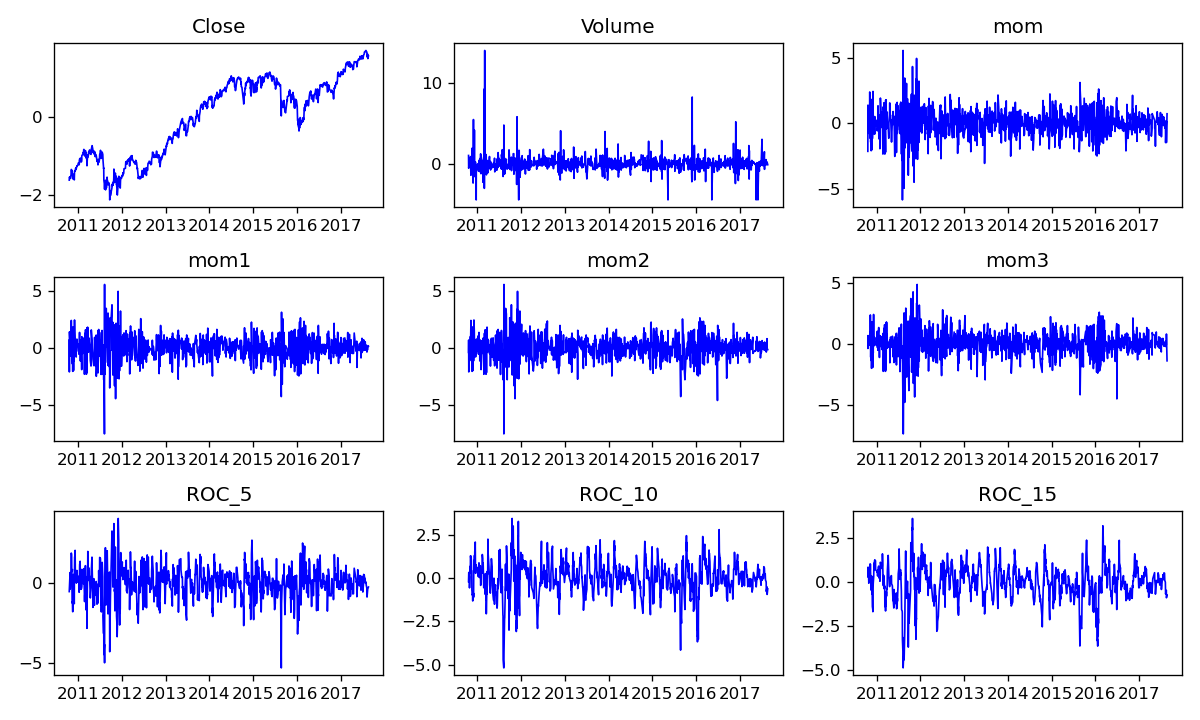
\includegraphics[width=\textwidth]{figures/Ass2/Ass2_Q4_standard_data.png}
    \end{minipage}
    \caption{The visualization of the first twelve columns. Columns were standardized.}
    \label{fig:Ass2_Q4_standard_data}
\end{figure}


\begin{table}[H]
\centering
\caption{The result of the \gls{ADF} on the dataset.}
\label{tab:Ass2_Q4_ADF_results}
{\tiny
\hspace*{-2cm}\begin{tabular}{lrrrrrrrrrrrr}
\toprule
{} &        Close &           mom &         mom1 &         ROC\_5 &        ROC\_10 &        ROC\_15 &        ROC\_20 &       EMA\_10 &       EMA\_20 &       EMA\_50 &      EMA\_200 &           Oil \\
\midrule
ADF Statistic               &    -1.085 & -12.134 &   -38.465 & -10.619 & -9.753 & -6.995 & -8.074 &    -0.967 &    -0.882 &    -0.791 &    -0.585 & -8.920 \\
p-value                     &     0.7 &  1.7e-22 &     0 &  5.5e-19 &  7.9e-17 &  7.5e-10 &  1.5e-12 &     0.7 &     0.7 &     0.8 &     0.8 &  1.0e-14 \\
\# Lags Used                  &     2 &  11 &     0 &  9 &  6 &  16 &  5 &     3 &     3 &     6 &     7 &  10 \\
\# Obs. Used &  1111 &  1102 &  1113 &  1104 &  1107 &  1097 &  1108 &  1110 &  1110 &  1107 &  1106 &  1103 \\
Critical Value (1\%)         &    -3.436 & -3.436 & -3.436 &    -3.436 & -3.436 &    -3.436 & -3.436 & -3.436 & -3.436 & -3.436 & -3.436 & -3.436 \\
Critical Value (5\%)         &    -2.864 & -2.864 & -2.864 &    -2.864 & -2.864 &    -2.864 & -2.864 & -2.864 & -2.864 & -2.864 & -2.864 & -2.864 \\
Critical Value (10\%)        &    -2.568 & -2.568 & -2.568 &    -2.568 & -2.568 &    -2.568 & -2.568 & -2.568 & -2.568 & -2.568 & -2.568 & -2.568\\
\bottomrule
\end{tabular}\hspace*{-2cm}
}
\end{table}

\textit{According to table \ref{tab:Ass2_Q4_ADF_results}, all columns were stationary except "Close price" and EMA\_X variables.  
We used a first-order differencing to turn these time series into the stationary data. Figures \ref{fig:Ass2_Q4_1diff_Close_signal} and \ref{fig:Ass2_Q4_PACF_ACF_1diff} indicate this $1^{st}$ order differencing for the "Close price" signal along with its \gls{ACF} and \gls{PACF} plots. These two plots also show that the data got stationary. Table \ref{tab:Ass2_Q4_ADF_results2} shows the ADF test on the $1^{st}$ order differencing variables.}

\begin{figure}[H]
    \centering
    \begin{minipage}[b]{1\textwidth}
        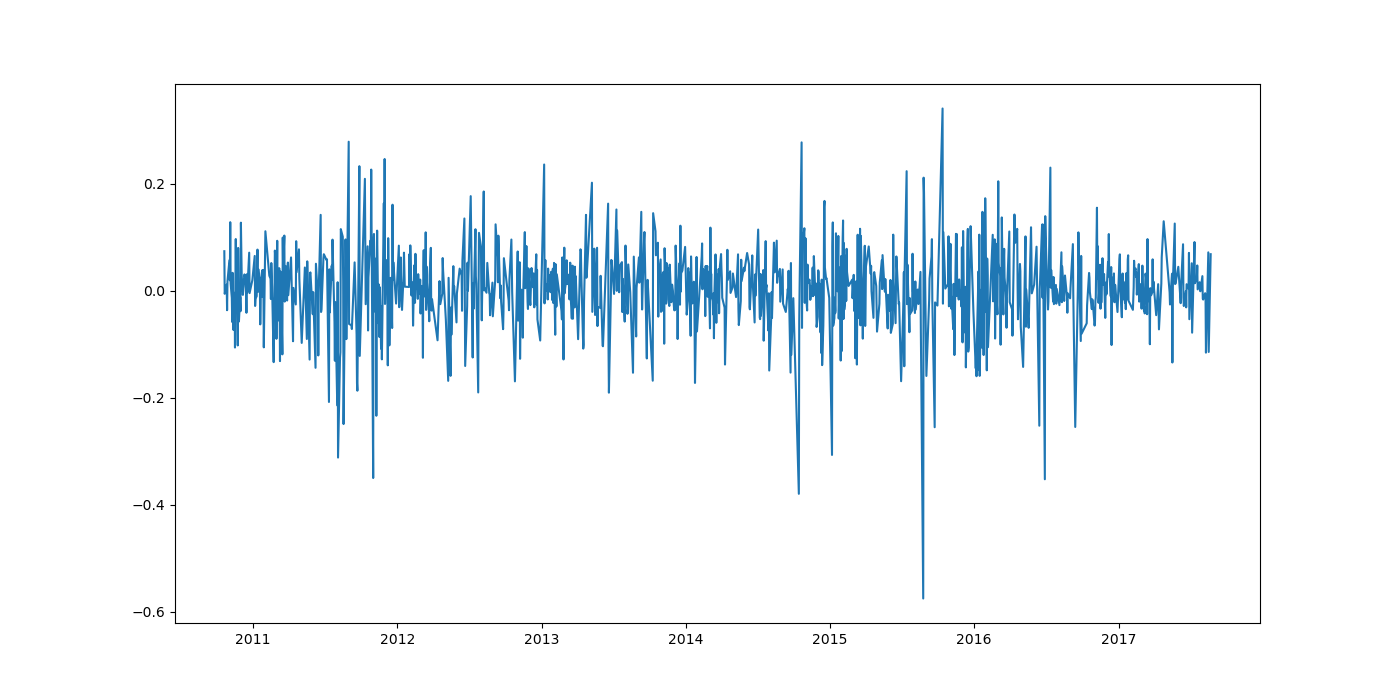
\includegraphics[width=\textwidth]{figures/Ass2/Ass2_Q4_1diff_Close_signal.png}
    \end{minipage}
    \caption{The $1^{st}$ order differencing of "Close price" data.}
    \label{fig:Ass2_Q4_1diff_Close_signal}
\end{figure}

\begin{figure}[H]
    \centering
    \begin{minipage}[b]{1\textwidth}
        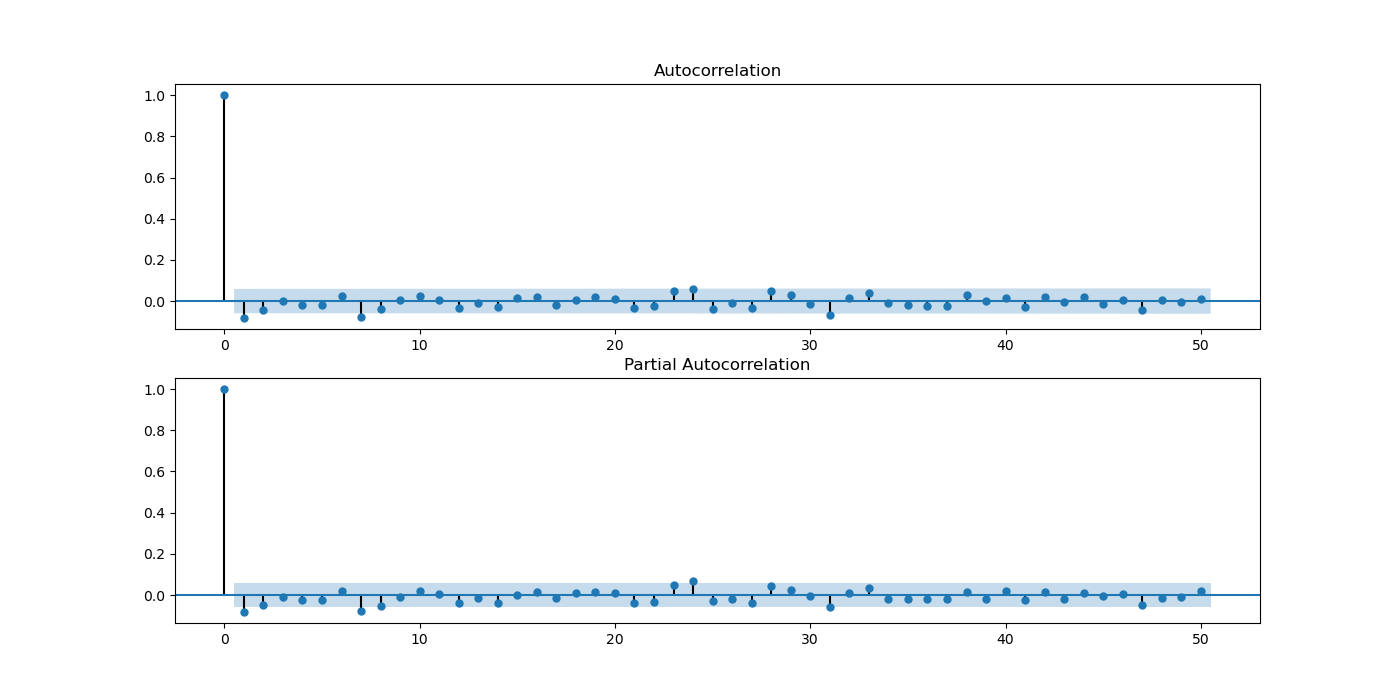
\includegraphics[width=\textwidth]{figures/Ass2/Ass2_Q3_PACF_ACF_1diff.png}
    \end{minipage}
    \caption{A plot of \gls{ACF} and \gls{PACF} on the $1^{st}$ order differencing in "Close price".}
    \label{fig:Ass2_Q4_PACF_ACF_1diff}
\end{figure}

\begin{table}[H]
\centering
\caption{The result of the \gls{ADF} on the $1^{st}$ order differencing variables.}
\label{tab:Ass2_Q4_ADF_results2}
{\tiny
\hspace*{-2cm}\begin{tabular}{lrrrrrrrrrrrr}
\toprule
{} &        Close &           mom &         mom1 &         ROC\_5 &        ROC\_10 &        ROC\_15 &        ROC\_20 &       EMA\_10 &       EMA\_20 &       EMA\_50 &      EMA\_200 &           Oil \\
\midrule
ADF Statistic               &   -25.69 & -12.13 &   -24.15 & -10.63 & -9.74 & -6.99 & -8.059 & -13.44 & -10.72 & -6.82 &    -4.72 & -8.91 \\

p-value                     &     0 &  1.7e-22 &     0 &  4.9e-19 &  8.1e-17 &  7.4e-10 &  1.6e-12 &  3.7e-25 &  3.0e-19 &  1.9e-09 &     7.6e-5 &  1.0e-14 \\
\#Lags Used                  &     1 &  11 &     1 &  9 &  6 &  16 &  5 &  2 &  2 &  5 &     6 &  10 \\
\# Observations Used &  1111 &  1101 &  1111 &  1103 &  1106 &  1096 &  1107 &  1110 &  1110 &  1.107 &  1106 &  1102 \\
Critical Value (1\%)         &    -3.436 & -3.436 & -3.436 &    -3.436 & -3.436 &    -3.436 & -3.436 & -3.436 & -3.436 & -3.436 & -3.436 & -3.436 \\
Critical Value (5\%)         &    -2.864 & -2.864 & -2.864 &    -2.864 & -2.864 &    -2.864 & -2.864 & -2.864 & -2.864 & -2.864 & -2.864 & -2.864 \\
Critical Value (10\%)        &    -2.568 & -2.568 & -2.568 &    -2.568 & -2.568 &    -2.568 & -2.568 & -2.568 & -2.568 & -2.568 & -2.568 & -2.568\\
\bottomrule
\end{tabular}\hspace*{-2cm}
}
\end{table}


\textit{After transforming and making stationary, we needed to find the best-fitted model. Thus we searched on various orders. For the searching area, we used all lags between 1 and 50. Figure \ref{fig:Ass2_Q4_AIC_plot} shows the \gls{AIC} over the different orders. The best order in terms of \gls{AIC} belonged to order 9 (VAR(9) model). We could do the same procedure to find the best order based on other information criteria. The below table shows the result of other information criteria.}

\begin{table}[H]
\centering
\caption{The result of other information criteria.}
\label{tab:Ass2_Q4_criteria}
\begin{tabular}{rlc}
\toprule
\# &  Information Criteria &   Best order \\
\midrule
1 & AIC  &  9 \\
2 & BIC  &  3\\
3 & FPE  &  9\\
4 & HQIC &  5\\
\bottomrule
\end{tabular}

\end{table}


\begin{figure}[H]
    \centering
    \begin{minipage}[b]{1\textwidth}
        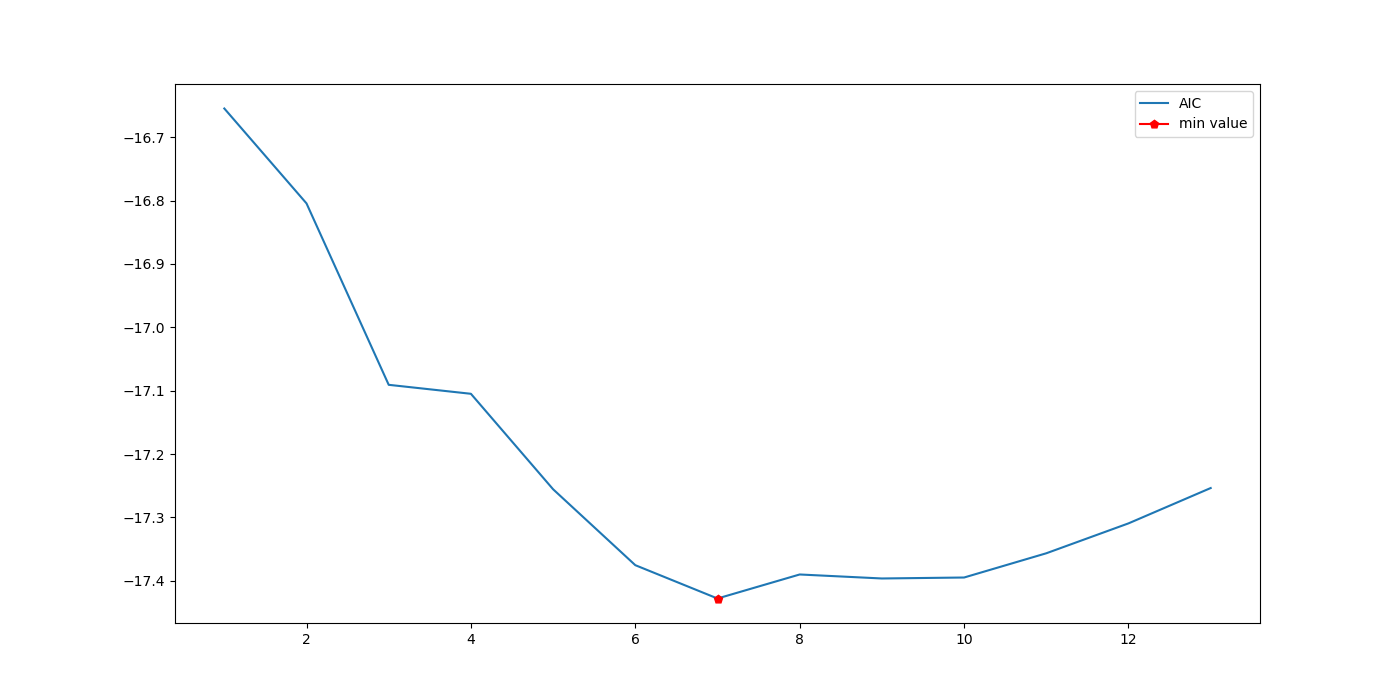
\includegraphics[width=\textwidth]{manuscript/src/figures/Ass2/Ass2_Q4_AIC_plot.png}
    \end{minipage}
    \caption{The \gls{AIC} over the different orders of VAR model.}
    \label{fig:Ass2_Q4_AIC_plot}
\end{figure}

\textit{Figure \ref{fig:Ass2_Q4_residual_plot} indicates the residual of the fitted model only for the first variable. As this plot illustrates, the residual signal of the model had a Gaussian distribution with zero mean. Besides, the \gls{ACF} plot shows that this signal was stationary.}



\begin{figure}[H]
    \centering
    \begin{minipage}[b]{0.8\textwidth}
        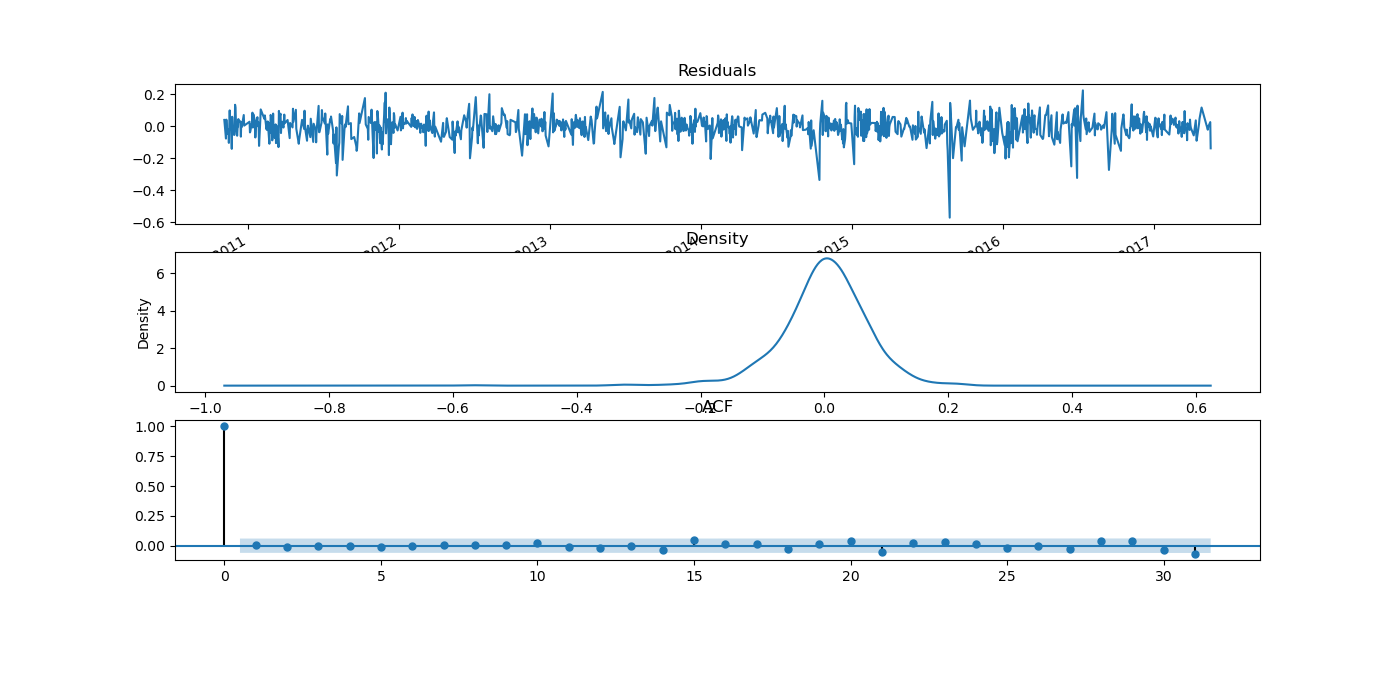
\includegraphics[width=\textwidth]{manuscript/src/figures/Ass2/Ass2_Q4_residual_plot.png}
    \end{minipage}
    \caption{The residual of the fitted model.}
    \label{fig:Ass2_Q4_residual_plot}
\end{figure}


\textit{In addition, we applied the Durbin Watson test to estimate the correlation between residuals. This correlation shows whether or not the pattern has any leftover in the residuals. As table \ref{tab:Ass2_Q4_DW_results} indicates Durbin Watson's results were close to 2. It means there was no correlation between residuals. } 

\begin{table}[H]
\centering
\caption{The result of Durbin Watson test on the dataset.}
\label{tab:Ass2_Q4_DW_results}
\begin{tabular}{rll}
\toprule
\# &  Variable Name &   The result \\
\midrule
1 & Close   &   1.99\\
2 & mom     &   1.98\\
3 & mom1    &   2.0\\
4 & ROC\_5   &   1.99\\
5 & ROC\_10  &   1.99\\
6 & ROC\_15  &   1.97\\
7 & ROC\_20  &   1.97\\
8 & EMA\_10  &   2.0\\
9 & EMA\_20  &   2.0\\
10 & EMA\_50  &   2.0\\
11 & EMA\_200 &        2.0\\
12 & Oil     &    2.0\\
\bottomrule
\end{tabular}




\end{table}




\textit{To forecast, we split data into test and train set like the last two parts. After prediction, we reversed differencing and standardization to get the real forecast. Figure \ref{fig:Ass2_Q4_Forecast_vs_Actuals_of_close} demonstrates the output of the fitted model only for "Close price." As can be seen, although the model could predict perfectly at the first, it got a flat slope. The RMS error for this model was 339.599.} 


\begin{figure}[H]
    \centering
    \begin{minipage}[b]{1\textwidth}
        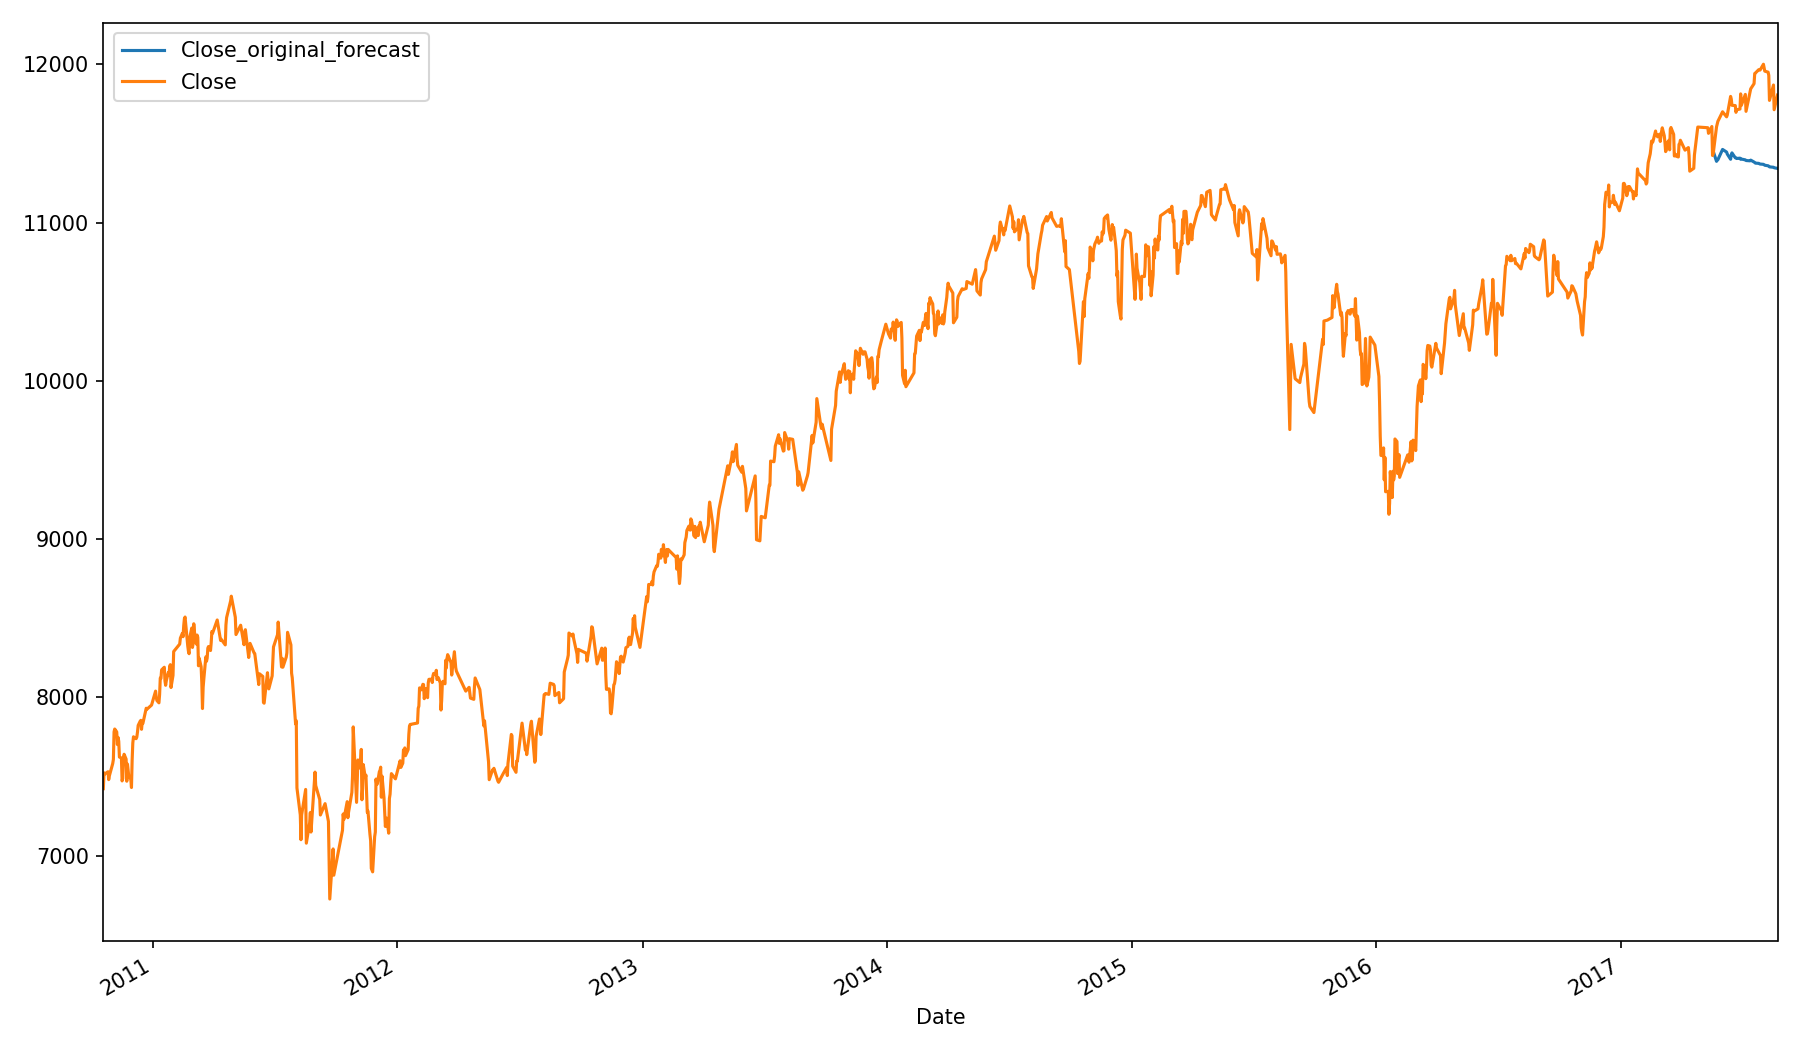
\includegraphics[width=.9\textwidth]{manuscript/src/figures/Ass2/Ass2_Q4_Forecast_vs_Actuals_of_close.png}
    \end{minipage}
    \caption{The prediction and actual data of VAR model.}
    \label{fig:Ass2_Q4_Forecast_vs_Actuals_of_close}
\end{figure}




\textit{For the rolling window approach, we used the same procedure in question 2. Figure \ref{fig:Ass2_Q4_Rolling_Forecast_vs_Actuals_of_close} demonstrates the output of the rolling window model for VAR. As can be seen, the model could follow the test set better than the previous models. The RMS error decreased from 339.599 to 117.565.}


\begin{figure}[H]
    \centering
    \begin{minipage}[b]{1\textwidth}
        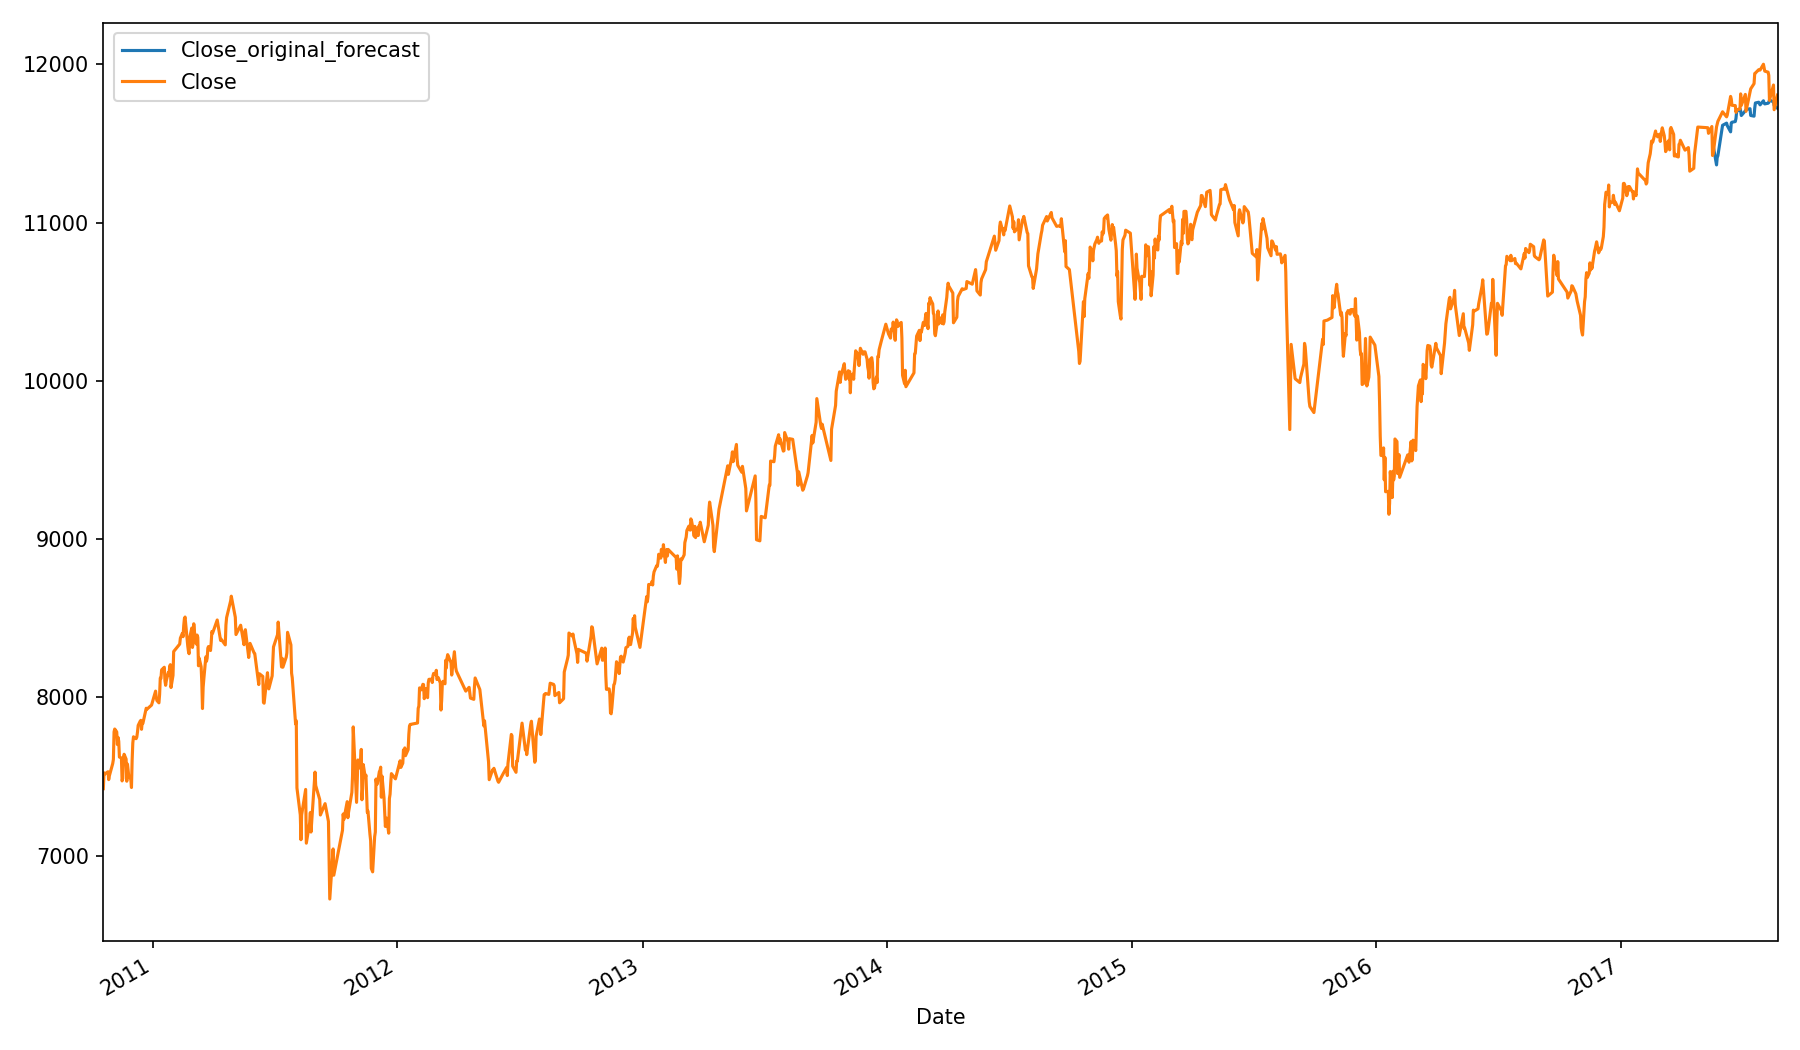
\includegraphics[width=\textwidth]{manuscript/src/figures/Ass2/Ass2_Q4_Rolling_Forecast_vs_Actuals_of_close.png}
    \end{minipage}
    \caption{The prediction and actual data of VAR model.}
    \label{fig:Ass2_Q4_Rolling_Forecast_vs_Actuals_of_close}
\end{figure}
%%%%%%%%%%%%%%%%%%%%%%%%%%%%%%%%%%%%%%%%%%%%%%%%%%%%%%%%%%%%%%%%%
%%%%%%%%%%%%%%%%%%%%%%%% Question 4 %%%%%%%%%%%%%%%%%%%%%%%%%%%%%
%%%%%%%%%%%%%%%%%%%%%%%%%%%%%%%%%%%%%%%%%%%%%%%%%%%%%%%%%%%%%%%%%
%\newpage
%\item \textbf{Summarize your findings and observations briefly in a final discussion. Submit both the developed code and your document to the Assignment 1 folder on D2L.}

\textit{All files were uploaded on my GitHub repository \cite{}. The below table, shows the important paths of the project. Beside the codes are available in Appendix }

\begin{table}[H]
\centering
\begin{tabular}{|l|l|}
\hline
\multicolumn{2}{|l|}{The Important Paths:        } \\ \hline
\ \ \ \    ./EE6563/Dataset/Ass1             & Assignment datasets\\ \hline
\ \ \ \    ./EE6563/code/Ass1/sun.py         & Assignment code\\ \hline
\ \ \ \    ./EE6563/code/Ass1/Temp.py        & Assignment code\\ \hline
\ \ \ \    ./EE6563/manuscript/src/figures   & Assignment figures\\ \hline
\ \ \ \    ./EE6563/manuscript/src/tables    & Assignment table\\ \hline
\ \ \ \    ./EE6563/manuscript/src/Ass1.tex  & Assignment document\\ \hline
\end{tabular}
\end{table}












\end{enumerate}



\newpage
\section*{REFERENCES}
\label{sec:sec6}
\printbibliography[heading=none]

%\bibliography{references}


\newpage
\section*{Appendix (codes)}
\subsection*{The script of sun.py}

\begin{lstlisting}
"""https://www.machinelearningplus.com/time-series/time-series-analysis-python/"""
import warnings

warnings.filterwarnings("ignore")

import math
import os

import matplotlib.pyplot as plt
import numpy as np
import pandas as pd
import statsmodels.api as sm

from pandas.plotting import lag_plot
from sklearn.linear_model import LinearRegression
from sklearn.metrics import mean_squared_error
from statsmodels.graphics.tsaplots import plot_acf, plot_pacf
from statsmodels.tsa import seasonal, stattools
from statsmodels.tsa.ar_model import AutoReg
from statsmodels.tsa.arima_model import ARIMA

\end{lstlisting}
\subsection*{The script of Temp.py}
\begin{lstlisting}
"""https://www.machinelearningplus.com/time-series/time-series-analysis-python/"""
import warnings

warnings.filterwarnings("ignore")

import math
import os

import matplotlib.pyplot as plt
import numpy as np
import pandas as pd
import statsmodels.api as sm
import seaborn as sns

from pandas.plotting import lag_plot
from sklearn.linear_model import LinearRegression
from sklearn.metrics import mean_squared_error
from statsmodels.graphics.tsaplots import plot_acf, plot_pacf
from statsmodels.tsa import seasonal, stattools
from statsmodels.tsa.ar_model import AutoReg
from statsmodels.tsa.arima_model import ARIMA


\end{lstlisting}

\end{document}